
\chapter{Úvod}
Bezpilotní letadla neboli drony, které se vyvíjeli dlouhá léta pro vojenské účely se staly poměrně novým trendem na poli civilního letectví. Drony se čím dál častěji používají v oblasti profesní činnosti, která často zahrnuje operace poblíž zástavby a lidí. S touto činností se pojí rizika, která se mají minimalizovat za pomocí předpisů a legislativ. Dodržovaní těchto předpisů a zásad však mnohdy není přímočaré. Proto se tato práce zabývá experimentální metodou vizualizace letových dat dronu v prostředí rozšířené virtuální reality, která má za úkol poskytnout prostředky pro zvýšení bezpečnosti, usnadnění pilotáže a zpříjemnění používání dronů. Práce rovněž adresuje problematiku autonomních režimů pilotáže dronu a snaží se zjednodušit programování a vykonávání misí dronů. 

Práce má experimentální charakter a začíná kapitolou o rozšířené realitě. V rámci kapitoly bude představen pojem "rozšířená realita" s drobným historickým přesahem. Dále budou detailně popsány brýle Hololens 2, které byly použity jako platforma implementovaného programu. Popis zahrnuje popis silných a slabších stránek brýlí, které byly vzaty v potaz ve vývojové fázi rozhraní. 

V další kapitole dojde k obeznámení s drony a to včetně prostředků k jejich ovládání. Dále jsou probrány legislativní omezení při provozování dronů spolu se zásadami pro bezpečné užívání dronů. Konec kapitoly je věnován analýze typického užití dronů. 

Poté se  práce již práce bude zaobírat samotným vývojem aplikace. Rozebrán bude návrhový proces, který byl zahájen analýzou předcházejících prací na toto téma, která je zakončena požadavky na nové řešení. V závěru kapitoly se nachází sada drátových a grafických modelů rozhraní, které mají za úkol vizualizovat prvotní rysy řešení. 

Vývojová část dále pokračuje samotnou implementací řešení. Vstup do kapitoly tvoří popis celé architektury, v které projekt figuruje. Pokračuje se představením softwarových nástrojů pro tvorbu programu. Zbytek kapitoly je věnován popisu průběhu implementačnímu procesu, který je rozdělen dle jednotlivých komponent programu. Závěr kapitoly tvoří optimalizační podkapitola.

Výslednou aplikaci autor v závěr podrobil rozsáhlému testování v rámci modelových scénářů, které byly vytvořeny na základě reálného profesního užití dronů. Z tohoto testování poté vychází závěr práce spolu s zhodnocením cílů daných v návrhové části práce. Závěr předchází drobná rozprava o budoucích směrech v rámci probírané problematiky.


\chapter{Rozšířená realita}
Rozšířená realita (augmented reality zkráceně AR) na rozdíl od virtuální reality (zkráceně VR), která umístí uživatele do plně vygenerovaného prostředí, má za cíl promítat informace/objekty do skutečného fyzického prostředí okolo uživatele. Tím vyplňuje mezeru mezi světem skutečným a světem virtuálním  \cite{Kniha2SchmalstiegDieter2016Ar:p}. 

\subsubsection[Pohled do historie]{Stručný pohled do historie\footnote{Odstavec je inspirován článkem \cite{historyAr}.}}
 První velký průlom v odvětví AR nastal v 60. letech a to projektem "Sword of Damocles". Jednalo se o první náhlavní displej, který byl zavěšen mechanizmem u stropu. Umožňoval monitorování pohybu hlavy a očí. Díky tomu mohl software korigovat zobrazované snímky. Přístroj sloužil k demonstraci konceptu a nenabízel moc velkou variabilitu \cite{Kniha1GreengardSamuel2019Vr}.

K praktickému užití AR došlo nejdříve v armádě, kde bylo nejprve použito pro výcvik pilotů v simulovaném prostředí. Armáda se dále zasloužila o integraci AR na palubu letounů a to zejména ve formě průhledových displejů (takzvaných HUD displejů). Prosazení plného syntetického vidění je spojováno s prototypem záchranné kosmické lodi X-38, kterou vyvinula NASA. Tento stroj byl vybaven displejem s rozšířenou realitou, který měl zastupovat přední okno tohoto kosmoplánu\cite{delgado2001hybrid}. Jak HUD displeje, tak syntetické displeje lze dnes běžně nalézt na palubě moderních civilních letounů.

K hromadnému používání AR v civilní sféře začalo docházet hlavně po roce 2000, začátkem je často označován rok 1998, kdy byla poprvé použita virtuální "First Down" čára v živém přenosu amerického fotbalu. Osobní užití AR je spojeno s nástupem chytrých mobilních zařízení a to ve formě aplikací, které do záznamu z kamery vkládaly užitečné informace. Příkladem tohoto principu v praxi může být aplikace MARTA od firmy Volswagen, která pomáhala technikům provádět opravy vozidel \cite{MartaArt} nebo kdysi populární hra Pokemon-Go.

První rozsáhlé nasazení AR ve formě brýlí však přišlo až v roce 2014 a to představením průlomového komerčního produktu pojmenovaného Google Glass. Brýle již byly dostatečné výkoné pro provoz bez přídavných výpočetních jednotek a zároveň jejich váha neomezovala uživatele v pohybu.
Produkt si kladl za cíl provést provázání s mobilními telefony a posloužit tak k podobnému účelu jako dnešní chytré hodinky. Zobrazení obrazu zajišťoval průhledový displej ve formě skleněného kvádru vložený před pravé oko. Na tomto displeji byly zobrazované informace do prostoru ve formě 2D karet, které připomínaly aplikace v telefonu. Interakce s brýlemi probíhala pomocí dotykového trackpadu na straně brýlí a hlasových povelů. Koncept se bohužel neujal a není nadále rozvíjen \cite{GoogleGlass}.

\section{Microsoft Hololens 2} \label{sec:Hololens}
První veřejně dostupné zařízení umožňující plné zasazení do argumentovaného 3D prostoru přinesla až první generace brýlí Hololens, které umožňuje zobrazení hologramů 3D objektů v prostoru se kterými lze za pomocí senzorů monitorující okolí brýlí přirozeně interagovat. 

Druhá generace se od první liší výrazně lepšími specifikacemi a přidanými funkcemi. Zásadní změnou  byl přechod z 32 bitové architektury x86 na platformu ARM, která nabízí lepší využití napájecího výkonu (proto se ve velkém využívá zejména u mobilních zařízení). Dalším vylepšením byly nové průhledové displeje, který nyní pokrývají až 52° zorného pole oproti původním 30°. Zvýšeno bylo také rozlišení těchto displejů. Mezi nové funkce patří eye tracking nebo-li sledování pohybu očí \cite{hololens1/2difrences}.

Brýle jsou prodávány ve třech edicích: normální, Industriální a Trimble XR10. Industriální edice se liší zejména podporou industriálních standardů, které umožňují užití brýlí na místech, kde je vyžadována vysoká čistota nebo kde jsou jiné nebezpečné podmínky (například biologické laboratoře nebo továrny na čipy. Edice Trimble XR10 umožňuje montáž na stavařskou helmu a určena na práci ve špinavých a hlučných pracovních oblastech \cite{hololens2msOptions}.

\subsubsection{Popis hardwarového vybavení Hololens 2}
Popis se vztahuje k obrázku \ref{pic:hololens2}. Brýle se na hlavu nositele připevňují pomocí prstence kolem hlavy a pomocného pásku přes hlavu (na zmírnění tlaku prstence na hlavu). Průměr prstence lze nastavit kolečkem na zadní části brýlí. Zde se také nachází baterie s napájecím konektorem a tlačítkem na zapínání. V zadní části jsou také vedeny antény pro Wi-Fi a Bluetooth. Po stranách prstence na oblastí ucha jsou přítomny reproduktory. 

Přední část brýlí je celá připevněna na mechanickém rameni. To slouží ke zvednutí brýlí, pokud nejsou  potřeba. V horní části se v pruhu nad průhledovou částí nachází několik senzorů. Jsou zde umístěny 4 kamery pro sledování pohybu hlavy, jedna RGB kamera, jedna kamera pro měření vzdáleností a 3 mikrofony. Nad tímto pruhem se nachází hlavní základová deska, ve které jsou hlavní výpočetní jednotky.

Průhledová část tvoří dutý ochranný plast, do kterého je zasazen průhledový displej. Na ten je promítáno za pomocí projektorů, které jsou také v pruhu s kamerami. V tomto plastu jsou u části styčné s nosem umístěny kamerky na snímání pohybu očí.\cite{hololens2ms}.
\begin{figure}[ht] %to do: udělat popisky česky
	\centering
	\includegraphics[width=\textwidth]{obrazky-figures/ar/hololensDescription.png}
	\caption{Rozebrané brýle Hololens 2 s popisky jednotlivých částí. Převzato z \cite{hololens2ms}.}
	\label{pic:hololens2}
\end{figure}


\subsubsection{Modalita/vstup od uživatele}
S rozhraním v brýlích se dá interagovat několika způsoby. Autor je seřadil podle obvyklé frekvence užití v aplikacích.
\begin{enumerate}
    \item Gesta a pohyb rukou -- Jedná se o hlavní cestu pro interakci s prostředím. Brýle dokáží rozpoznat přesný pohyb rukou včetně pohybu prstů. Díky tomu lze provádět různá gesta v prostoru a tím interagovat s okolím. Ovládání je velmi intuitivní, protože můžete na jednotlivé objekty "fyzicky sahat". Pokud  aplikace emuluje gravitaci, můžete z objekty i házet či jinak užívat fyzické vlastnosti objektů. Ukázka této funkcionality je na obrázku \ref{pic:hololens2Demo}. S objekty lze interagovat i na dálku.
   \item Pohyb v prostoru a pohyb hlavy -- Rozhraní lze naprogramovat, aby interakce s prostředím probíhala díky pohybu uživatele v prostoru. Lze tedy implementovat, aby jednotlivé objekty reagovaly například při pohledu na objekt. 
    \item Hlasové ovládání -- Díky integrovaným mikrofonům a jednotce pro rozpoznávání řeči lze brýle ovládat hlasovými příkazy. Syntezátor hlasu naopak může k uživateli promlouvat díky integrovaným reproduktorům v zadní části brýlí.
    \item Pohyb očí -- Díky snímání pohybu očí může například rozhraní reagovat při pohledu na určitý objekt. Při testování autor shledal, že je pohyb očí zaznamenán poměrně přesně. Pro jemnou interakci však nestačí.
 
    \item Externí zařízení -- I když brýle lze užívat pouze za pomocí výše zmíněného, uživatel má možnost si pomocí Bluetooth a Wi-Fi připojit vlastní periferie, jako je klávesnice, myš nebo třeba gamepad. 
\end{enumerate}
\begin{figure}[ht] 
	\centering
	\includegraphics[width=0.95\textwidth]{obrazky-figures/ar/hololensDemo.png}
	\caption{Ukázka ovládání scény za pomocí gest. Převzato z video dema \cite{hololens2videoDemo}.}
	\label{pic:hololens2Demo}
\end{figure}

\subsubsection{Souhrn technických limitací brýlí}
Brýle obsahují velmi pokročilý hardware, který velmi dobře zasazuje uživatele do augmentované reality. Tato technologie má však své limitace, které musel brát autor v potaz při tvorbě práce. Poznatky byly zjištěny experimentálně. 
\begin{itemize}
    \item Malé zorné pole -- I když byl rozsah zorného pole vylepšen, je pořád velmi malý - 52°.  Zdroj \cite{HumanEye} uvádí, že je člověk schopen vnímat až 190° v horizontálním rozsahu a 100° vertikálním rozsahu. Z toho plyne, že je nutné rozhraní nutné smrštit co ke středu pomyslné zorné linie. Užít vizualizace v periferní vidění je tedy proto nemyslitelné. Vizualizace omezení je na obrázku \ref{pic:hololens2Fov}.
    \item Nepřítomnost GPS modulu -- Brýle nemají žádnou jednotku pro lokalizaci uživatele. Při spuštění brýlí je uživatel umístěn na nulové souřadnice. Z toho vyplývá, že brýle využívají vlastní souřadnicový systém. Implementovaný program tedy musí provádět kalibrace pro správnou lokalizaci uživatele.
    
    \item Platformní limitace - Při vývoji programu lze užít pouze omezené množství programových knihoven. Tento fakt je způsobem díky nezvyklé kombinaci  architektuře ARM a implementační platformy UWP (Univerzal Windows Platform).

    \item Mapování prostoru -- Brýle neobsahují žádnou databázi o podobě okolí. Okolí si brýle modelují za pomocí kamer a to pouze ve velmi blízkém okolí (cca rádius 10m od uživatele). Toto okolí nemusí být vytvořeno dokonale a tudíž se na něj nelze spolehnout. Pro využití v kontextu vizualizace dronu je velmi limitující.
    \item Konektivita -- brýle mají integrovaný Wi-Fi a Bluetooth modul. Pouze za pomocí těchto technologií lze brýle připojit k dalším zařízením. Použití Bluetooth komunikace by v práci vedla na velkou implementační náročnost, které neodpovídá povaha projektu, proto bude komunikace přes Wi-Fi modul preferována. Wi-Fi na více podporuje lepší přenosové rychlosti a lepší variabilitu. 
    
    Wi-Fi modul nelze užít jako přístupový bod (zkratka AP), což brýle odsuzuje k závislosti na externím Wi-Fi AP. Při vývoji proto bude nutné počítat s přítomností tohoto hotspotu. 
\end{itemize}
\begin{figure}[ht] 
	\centering
	\includegraphics[width=0.85\textwidth]{obrazky-figures/ar/Hololens-2-fov.png}
	\caption{Ukázka limitace zorného pole. Převzato z \cite{hololens1/2difrences}}
	\label{pic:hololens2Fov}
\end{figure}

\chapter{Drony a jejich použití }
Drony, formálně pojmenované UAV (unmanned aerial vehicle), jsou obecně letadla bez pilota, posádky či pasažérů na palubě letounu. Tento letoun je pak řízen dálkově či může být řízen plně autonomně palubním počítačem \cite{UAVMeaning}. 

Koncept dronů sahá až do 19 století, kde bylo poprvé  zaznamenáno jejich nasazení. Jednalo se o horkovzdušné balóny vybavené výbušninami, které byly shazovány za pomocí časové zápalky (viz. obrázek \ref{pic:balon}). Roku 1839 Rakousko použilo tuto zbraň při útoku na Benátky. Velký průlom v této oblasti byl zaznamenán v první světové válce, kdy vznikl "Hewitt-Sperryův automatický letoun", jeden z prvních radiem ovládaných letounů (viz. obrázek \ref{pic:autoPlane}). Další velký pokrok přišel v druhé světové válce, kdy drony začaly ukazovat svůj velký potenciál jak na bojišti, tak v tréningových oblastech pro výcvik.

Přestože bylo za války vyrobeno nepřeberné množství těchto dronů, lidé byly kvůli jejich špatné spolehlivosti velmi skeptičtí, což vedlo ke zpomaleni vývinu a tak další pokrok přicházel až v době války ve Vietnamu a během studené války. \cite{DroneHistory,DroneHistory2WWX,DroneKatogorySouhrn,DroneHistory3} 

Tato historie se spíše stahovala k vývoji bezpilotním letounům (to jsou motorové letadla těžší než vzduch, používající ke svému pohybu aerodynamických sil, s pevnými nosnými plochami). Drony pro civilní použití, jak je známe dnes jsou však spíše multi-rotorové stroje. První pokus o vytvoření takovéhoto stroje se připisuje designérovy Louis Breguetovy, jenž navrhl první takovýto stroj (viz. obrázek \ref{pic:quadrocopter}). Po sestavení stroje bylo poznamenáno, že stroj několikrát letěl \cite{Quadcopter}. Rozšířené užití designu multi-rotorové stroje  na poli civilním trhu s drony je dle zdroje \cite{DroneHistory3} zaznamenáno v prvním desetiletí 21. století. Od těchto dob se technologie dronů neustále vyvíjí a to především  v oblasti pohodlnosti použití, spolehlivosti a levnější výroby.


\begin{figure}[ht]
    \centering
    \begin{subfigure}[t]{0.27\linewidth}
        \centering
        \includegraphics[width=\linewidth]{obrazky-figures/drony/history-of-drones-balloons.jpg}
        \caption{Ilustrace nejstarších dronů. Převzato z \cite{DroneHistory}.}
        \label{pic:balon}
    \end{subfigure}
    \hfill
    \begin{subfigure}[t]{0.26\linewidth}
        \centering
        \includegraphics[width=\linewidth]{obrazky-figures/drony/hewitt-sperry_automatic_airplane_1918.jpg}
        \caption{Hewitt-Sperryův automatický letoun. Převzato z \cite{DroneHistory2WWX}.}
        \label{pic:autoPlane}
    \end{subfigure}
        \hfill
    \begin{subfigure}[t]{0.43\linewidth}
        \centering
        \includegraphics[width=\linewidth]{obrazky-figures/drony/Bothezat_Quadrotor.jpg}
        \caption{Quadrokoptéra de Bothezat helicopter. Převzato z \cite{Quadcopter}.}
        \label{pic:quadrocopter}
    \end{subfigure}
    \caption{Průlomové historické stroje v oblasti technologie dronů.}
    \label{pic:historymisc}
\end{figure}


\section{Moderní civilní drony} \label{sec:modCivDrony}
Jak již bylo řečeno, na civilním trhu dronů nejčastěji nalezneme multirotorové stroje, nejčastěji 4 rotorové kvadrokoptéry. Vyrábějí se i více rotorové varianty drony, které mohou díky přidaným rotorům poskytnout větší zvedací výkon a redundanci pro případ selhání jednoho či více pohonných systémů \cite{Multirotor}. 

Multirotorový design je v oblasti dronů oblíbený, protože umožňuje kolmý start a vznášení se namístě. Zároveň nevyžaduje složité mechanizmy, jako je cyklika a kompenzační rotory jako je tomu u klasických vrtulníků. Každá pohonná jednotka dronu je identická a ovládání dronu je uskutečněno díky regulaci výkonu jednotlivých rotorů. I když jsou pohonné jednotky identické, pro vyrušení nežádoucích rotačních momentů je potřeba zajistit, aby sousední rotory měli vrtule s obráceným stoupáním a otáčeli se opačně (proto málo kdy naleznem drony s lichým počtem rotorů)\cite{Quadcopter}. Obrázek dronu užitého při vývoji viz. \ref{pic:mavicMini}.

Jelikož je potřeba rychle regulovat výkony motorů pro korektní řízení dronu, je ideálním kandidátem pro pohon elektrický proud. Jeho dodávku obvykle zajišťuje akumulátor Li-Po nebo Li-Ion. Tyto akumulátory by měly být ohodnoceny vysokou hodnotou C (tato hodnota značí jaké množství energie je schopna bezpečně dodat) \cite{bateriesDron}.

Udržení dronu stabilně ve vzduchu je složitý úkol, proto dron disponuje sadou senzorů, mezi nejnutnější patří gyroskop a akcelerometry (celý systém se nazývá IMU) s jejichž pomocí je možné dron stabilizovat. Pro přesné držení polohy dron na více potřebuje přijímač GPS, elektronický kompas a výškoměr. Výškoměr je obvykle u dronů optický, kvůli nízkým pořizovacím nákladům. U dražších dronů můžeme nalézt i barometr. Optické čidlo může být také využito pro korekci polohy dronu, jako je tomu u dronu DJI. Optická čidla se navíc nově používají pro detekci překážek. Kvůli těmto optickým senzorům se nedoporučuje létat s dronem za snížených viditelnostních podmínek. Pro správnou funkci potřebují čidla před letem zkalibrovat, často tak budete muset provádět kalibraci kompasu a jednotky IMU. Výstupy těchto senzorů spolu se vstupy od uživatele z vysílačky jsou následně zpracovány letovým počítačem a výstupem jsou úrovně výkonu pro jednotlivé regulátory motorů \cite{droneSenzors}.

Moderní drony z pravidla obsahují kameru pro nahrávání a přenos obrazu směrem k pilotovy. Tato kamera může být fixně umístěná - tuto variantu nalezneme například u FPV dronů. Druhou častější variantou je upevnění kamery do gimbal stativu, který stabilizuje kameru, aby výsledný obraz byl plynulý a vyhlazený. Často je tento mechanizmus obohacen o optickou stabilizaci, pro ještě lepší požitek z videa. Tato jednotka se u menších dronů nachází ve předu dronu. U filmařských dronů se tato jednotka nachází na spodku dronu přesně ve středu dronu a to z důvodu váhy kamery, která by dronu mohla destabilizovat. Tento design obvykle doprovází zvedací podvozek, aby nezavázel ve scéně kamery.


\begin{figure}[h]
  \begin{minipage}{0.5\textwidth}
    \centering
    \includegraphics[width=\textwidth]{obrazky-figures/drony/djiMavicMiniPopis.jpg}
    \caption{Ukázka dronu Mavic Mini 2 \\využitého pro vývoj. Převzato z \cite{mavici2pic}.}
    \label{pic:mavicMini}
  \end{minipage}
  \begin{minipage}{0.45\textwidth}
    \centering
    \includegraphics[width=\textwidth]{obrazky-figures/drony/DroneIntenals.png}
    \caption{Schéma zapojení součástek dronu. Převzato z \cite{droneIntrnals}.}
    \label{fig:dronSchema}
  \end{minipage}
\end{figure}

\section{Prostředky pro ovládání dronů} \label{sec:ovladace}
\subsubsection{Pákový ovladač}
V dnešní době se většina civilních dronů ovládá za pomocí 2 pákových joysticků neboli 4 os. Každá osa má přiřazený směr pohybu dronu dle zvoleného ovládacího módu (obvykle můžete módy přepínat v ovladači). Standardně se používají módy 4 (viz. obrázek \ref{pic:pakaMody}). Mód zde popsaný bude mód 2, protože se v kontextu dronů používá nejvíce. V tomto módu má levý joystick funkci zvyšování a snižování výšky ve vertikální ose. V horizontální ose se ovládá rotace dronu doleva/doprava. Pravým joystickem se ovládá pohyb v před/vzat na vertikální ose, pohyb doprava/doleva se ovládá na horizontální ose. Při pohybu joysticků do krajních poloh směrem k sobě dron odstartuje (pouze u dronů DJI).

Ovládání dronu je díky stabilizačním asistentům dronu jednoduché, pokud budou joysticky ve středové poloze, dron zastaví a bude se vznášet na místě. Rychlost reakce dronu na změny polohy pák se liší dle zvoleného módu letu. V mód Position dron jemně mění svou pozici, v módu Sport reaguje rázněji a létá vyššími rychlostmi. V posledním módu Cinematic dron létá velmi plynule.

Ovladač často obklopují pomocné ovládací prvky, na ovladači dronu použitého k vývoji je na vrchní straně ovladače přítomna sada dvou tlačítek. Jedno slouží pro návrat do oblasti vzletu, druhé slouží k zapnutí vysílače. Na zadní straně je přítomno tlačítko pro pořízení fotky a videa. Je zde také roller ovládající pohyb gimbalu ve vertikální ose. Hight-end ovladače obsahují i integrovaný displej pro zobrazení videa z dronu. Levnější tuto možnost poskytují přes připojený mobilní telefon. Příklad ovladače je na obrázku \ref{pic:paka}.
\begin{figure}[h]
  \begin{minipage}{0.55\textwidth}
    \centering
    \includegraphics[width=\textwidth]{obrazky-figures/drony/controler.jpg}
    \caption{Ovladač Mavicu Mini 2.\\ Převzato z \cite{pakaOvladac}.} % popsat obrázek
    \label{pic:paka}
  \end{minipage}
  \hfill
  \begin{minipage}{0.4\textwidth}
    \centering
    \includegraphics[width=\textwidth]{obrazky-figures/drony/transmiterMods.jpg}
    \caption{Módy pákového ovladače. Převzato z \cite{pakaMody}.} % to do zvětšit obrázek
    \label{pic:pakaMody}
  \end{minipage}
\end{figure}

\begin{figure}[h]
  \begin{minipage}{0.6\textwidth}
  \subsubsection{DJI Motion 2 }
    Jedná se o nový ovladač, který v kombinaci s brýlemi je určen pro řízení FPV dronů. Je specifický tím, že se dá ovládat pouze jednou rukou. Směr kupředu ovládáte spouští ovladače. Stoupání a zatáčení se ovládá náklonem ovladače. Dodatečné pohyby lze provést mini joystickem. Tento ovladač je zmíněn díky možnosti ovládání pouze jednou rukou, což by usnadnilo manipulaci s objekty v prostředí AR. 
  \end{minipage}%
  \hfill
  \begin{minipage}{0.38\textwidth}
    \centering
    \includegraphics[width=\textwidth]{obrazky-figures/drony/djiMotion.png}
    \captionsetup{type=figure} % Set up for figure caption outside of float
    \caption{Ovladač DJI Motion~2. Převzato z \cite{djiMotionPic}.}
    \label{fig:DjiMotion}
  \end{minipage}
\end{figure}
\newpage
\subsection{Softwarové vybavení \& stávající řešení}

\subsubsection{Lichi}

\paragraph{Plánování mise a uskutečnění mise}

\newpage

\section{Legislativa a pravidla pro civilní létání z drony}
V průběhu posledních let, zvláště od období masivního rozšíření dronů mezi širokou veřejnost došlo k značným úpravám v legislativě pro provoz dronů. Tyto nová nařízení měli zajistit bezpečnější provoz dronů ve veřejném vzdušném provozu a zajistit respektování občanského soužití. Tyto pravidla se musí při létání striktně dodržovat, aby se předešlo zbytečným nehodám a incidentům. Proto autor uznal za vhodné tyto pravidla nastudovat a rozebrat nejzásadnější body. Tento rozbor bude dále využit při návrhu aplikace. Rozbor je aktuální k začátku roku 2024.

\subsection{Kategorie dronů}
Provozování dronu se dle účelu použití dělí na 3 hlavní kategorie: Open, Specific a Certified. Tyto kategorie se liší hlavně rizikem použití. Nejvíce pozornosti bude věnováno kategorii Open, protože je nejvíce relativní k povaze práce.

\subsubsection{Specific}
Tato kategorie zahrnuje operace dronů se středním rizikem. Patří sem operace, které vyžadují prolomení limitací kategorie Open. Příkladem může být let bez přímé viditelnosti na dronu, let 120m nad zemí, odhození materiálu, překročení maximální letové hmotnosti 25 kg nebo lety s těžkými drony nad zástavbami\cite{EASA:SpecificCategory}. 
    
Pro tuto kategorii byly vytvořeny dva standardní scénáře užití, které nepotřebují autorizaci od AESA. Jedná se o scénář letu typu VLOS (létání při přímé viditelnosti na dronu) a BVLOS (létání bez přímé viditelnosti na dronu). Pokud aktivita nespadá do těchto scénářů je potřeba povolení od EASA \cite{DroneKatogorySouhrn,EASA:SpecificCategory}.  
    

\subsubsection{Certified} 
Kategorie zahrnuje vysoce rizikové použiti dronů. Do kategorie například patří provoz bezpilotních nákladních letadel, doručovací drony nebo vzdušné taxi. Jak název napovídá, všechny tyto aktivity musí být certifikovány od EASA \cite{EASA:CertifiedCategory}.

\subsubsection{Open} 
Tato sekce vzešla ze zdrojů \cite{EASA:openSouhrn2024,AlzaDronyKategorie,DroneKatogorySouhrn}. Kategorie Open je dostupná pro širokou veřejnost, určena je pro operace s nízkým rizikem. Na provoz dronu v této kategorii nepotřebujete povolení od organizace AESA. Kategorie Open se dále dělí na podkategorie A1, A2 a A3. Pro pilotáž dronů v kategorii A1/A3 se musíte registrovat na webu ÚCL (úřad civilního letectví) a absolvovat online školení. Pro kategorii A2 na více musíte mít certifikaci. V kategorii A2/A3 musíte mít sjednané povinné ručení dle podmínek kategorie.


Od roku 2024 každý nově prodaný dron musí být klasifikován do tříd C0-C4. Třídy lze přímo namapovat na podkategorie Open, ale je možné létat s dronem nízké kategorie podle pravidel vyšší kategorie (A3). Drony neoštítkované kategorií C, které byly prodány před rokem 2024 lze zařadit do třídy A1 pokud jejich letová hmotnost nepřesáhla 250g, jinak jsou zařazeny do kategorie A3.

Kategorizace slouží k minimalizování rizika střetu s osobami. Nad lidmi a v zástavbě můžete bez licence létat pouze s nejlehčími drony, s licencí můžete létat i s mírně těžšími drony. Provoz velmi těžkých dronů (>4 Kg) je možný pouze daleko od lidí a zástavby. 

\paragraph{Jednotlivé podkategorie Open:}
\begin{itemize}
    \item A1 -- s dronem se smí létat nad lidmi, ale nesmíte létat nad skupinami lidí. Do této kategorie spadají třídy C0 a C1. Pro pilotáž dronů v této kategorii se budete muset zaregistrovat na webu ÚCL a složit online test. Vyjmou jsou dětské hračky nevybavené kamerou. Tyto drony můžete provozovat také v kategorii A3.

    \item A2 -- s těmito drony nesmíte letět blízko lidí. Do této kategorie spadá třída dronů C2. Na tuto kategorii musíte absolvovat školení spolu s certifikačním procesem pro získání licence A2. Tato skupina je určená pro létání v zástavbě s těžšími drony.
    \item A3 -- do této kategorie automaticky patří všechny drony třídy C3 a výše (hmotnost do 25 kg), dále pak drony soukromě postavené a drony neoštítkované prodané před rokem 2024 s letovou hmotností nad 250g. S těmito drony musíte létat daleko od lidí a zástavby.
\end{itemize}

\paragraph{Jednotlivé třídy dronů:}
\begin{itemize}
    \item C0 -- Nejmenší drony (hmotnost do 250g) s maximální rychlostí do 68 km/h a napájením do 24V. Příkladem může být dron Mavic Mini 2 který byl použit pro vývoj. 
    \item C1 -- Drony vážící do 900g s maximální rychlostí do 68 km/h, napájením do 24V. Obsahují více bezpečnostních prvků než kategorie C0 a hluk je limitován 85 dB.
    \item C2 -- Drony vážící do 4 Kg, stejné povinné bezpečnostní prvky jako u C2, na více musí ale obsahovat Low Speed mode (3m/s), aby se mohl pohybovat v blízkostí lidí. Hlučnost je omezena do 97 dB a pohon je limitován 48 V.
    \item C3 -- Drony do 25 Kg a musejí se vejít do rozměru 3m. Pohon do 48 V.
    \item C4 -- Je určena pro modely letadel, stahuje se na ní pouze váhové omezení (<25Kg) a je zde zakázán autonomní režim. 
    \item C5/C6 -- Podobné C3 s přidanými bezpečnostními prvky.
\end{itemize}


\begin{figure}[ht]
	\centering
	\includegraphics[width=0.81\textwidth]{obrazky-figures/drony/droneCatTable.png}
	\caption{Přehledová tabulka kategorií dronů a podkategorií Open.  Zdroj \cite{EASA:openSouhrn2024}.}
	\label{covpitDrLiner}
\end{figure}


\subsection{Předstartovní procedura typického dronu}
Vývoj v oblasti dronů značně zjednodušil užívání dronů a proto pro mnohé uživatele navodil falešný pocit robustnosti dronů. Drony jsou i přes veškerá zjednodušení pořád velmi sofistikovaná a křehká zařízení, které je potřeba provozovat s respektem. Proto autor sepsal několikabodový checklist, který by zodpovědný operátor dronu měl dodržovat.  Procedura je psaná pro dron DJI Mavic Mini 2, ale není problém ho aplikovat na jiné typy dronů. Procedura vychází ze zdrojů \cite{PreflightChecklistPdf,PreflightChecklistSaftyCulture}, manuálu \cite{PreflightChecklistDJI} a zkušeností autora. 
\begin{enumerate}
    \item Ještě před vyražením do terénu aktualizujte veškerý firmware a letové databáze. Mějte v pořádku všechny legislativní dokumentace a dron mějte zaregistrovaný a oštítkovaný.
    \item Ujistěte se, že nechcete létat v bezletové/zakázané zóně. Pokud létáte poblíž letišť nebo v jiných podobných zónách, pravděpodobně budete muset mít sníženou maximální možnou letovou výšku na 80m. Autor však doporučuje, za těchto specifických okolností, v rámci bezpečnosti létat výrazně níže. Je doporučeno stanovenou maximální výšku zadat do vysílače. Chytřejší vysílače vás na tyto zóny obvykle upozorní. 
    \item Kontrola povětrnostních podmínek - Silnému větru je potřeba přizpůsobit let, poryvy větru mají často tendenci tlačit dron na blízké překážky. Na přistání je dobré si vyhradit větší prostor než obvykle.
    \item Kontrola teploty - Při mrazech způsobují fyzikální vlastnosti akumulátoru úbytek výkonu a je potřeba tento jev zohlednit.
    \item Fyzická kontrola stavu dronu - Je potřeba zkontrolovat zda-li se dron při přepravě a sestavení nepoškodil. Zejména autor doporučuje soustředit se na potencionální praskliny, které vznikají zejména v u kloubů ramen skládacích dronů. Dále je potřeba zkontrolovat stav vrtulí, často se stává, že vrtule je naprasklá nebo není pevně uchycena. Nekonzistentní stav vrtule může vést k roztrhnutí vrtule za letu. Poškozené vrtule bezprostředně vyměňte.
    \item Sundání aretace gimbalu kamery a kontrola volnosti pohybu gimbalu.
    \item Kontrola stavu baterie dronu - baterie by měla být při startu vždy plně nabita. Pokud tomu tak není, je potřeba tomuto faktu přizpůsobit plán letu. Napůl vybité baterie mají na více tendenci hned po startu znatelně snížit indikovanou úroveň nabití (prohlašuje autor na základě zkušeností).
    \item Spuštění vysílače a kontrola stavu baterie vysílače.
    \item Spuštění dronu a umístění dronu na rovný podklad. Nad a kolem vzletové oblasti by neměli být žádné překážky. Pokud startujete například pod střechou, riskujete, že dron v případě ztráty signálu přistane na střechu...
    \item Pokud dron potřebuje provést kalibraci IMU nebo kompasu, proveďte ji.
    \item Vyčkání na získání polohy z GPS jednotky. Po získání polohy provést kontrolu korektního nastavení takzvaného "home pointu" - to jest bodu na který se případně dron bude vracet v případě výpadku signálu. Pokud si to situace vyžaduje nastavte i bezpečnou návratovou výšku. Zároveň je dobré nastavit maximální výšku podle legislativních/územních omezení (obvykle 120m).
    \item Pokud plánujete létat v tmavém prostředí, ujistěte se, že dronu fungují poziční světla. 
    %\item Dron by měl být v tuto chvíli připraven k letu.
    
\end{enumerate}
\subsection{Základní pravidla pro létání z drony}
\newpage
\section{Užití dronů \& typické mise}


\chapter{Návrh řešení}
Tato sekce se věnuje návrhového procesu řešení. Návrhový proces začal analýzou a subjektivním zhodnocením původního řešení. Pokračuje se soupisem nejdůležitějším soupisem požadavků řešení. Splnění těchto požadavků bude testováno a zhodnoceno ke konci práce.

Po soupisu požadavků bude nastíněn prvotní návrh v podobě drátových modelů, odladěné modely budou následně přetvořeny do líbivějších grafických modelů, které budou zaměřeny kosmetickou část rozhraní.
\section{Analýza původních řešení}
Tato práce má vycházet na základě řady prací, z nichž poslední práce \cite{KyjacMartin2022Vnpp} dokázala pomocí proprietárního protokolu se propojit s telefonem připojeným do vysílače. Tento telefon za pomocí modifikované aplikace dokázal zasílat telemetrická data přímo do brýlí. V brýlích běžela aplikace, která dokázala za pomocí těchto data dronu správně umístit do scény. 

Dron byl následně zaměřen a ve směru od uživatele byl vykreslen obrazec složen ze dvou půlměsíců. Kolem tohoto půlměsíce byla vizualizualizovaná relativní výška (spolu se sloupcovým vizualizačním prvkem), vzdálenost od uživatele, indikace stavu baterie. Pod tímto eliptickým tvarem se nacházel 3D objekt dronu, která vizualizovala natočení dronu. Okolo byly prvky indikující blízkou překážku. Mezi poslední prvek patřila šipka indikující směr letu. Původní řešení je zobrazeno na obrázku \ref{pic:prevUiDesign} a \ref{pic:prevMisionObject}.

\subsubsection{Analýza metodiky sledování dronu}
Z testů dosavadního řešení vyplynulo následující zjištění. Ke sledování pohybu dronu mohly být využity data z GPS nebo z jednotky IMU (více o senzorech viz. sekce \ref{sec:modCivDrony}). V původní práci bylo doporučeno pro nejlepší výsledek doporučeno využít jednotku IMU. Autor však po testování zjistil, že kumulativní chyba po čase letu se zvedne na tolik, že vizualizace přestane pracovat korektně. Z tohoto důvodu se autor usoudil, že je oba přístupy nutné zkombinovat a tuto kumulativní chybu korigovat za pomocí jednotky GPS.

Jelikož brýle Hololens nemají jednotku GPS je na začátku relace potřeba dron zanést do souřadnicového systému pomocí procesu kalibrace, implementovaný proces autorovi nevyhovoval a proto se autor v implementační části zaměří na jeho zdokonalení/zjednodušení
\subsubsection{Analýza  vizualizace veličin a letových dat}
Původní rozhraní dokáže vizualizovat základní letové veličiny dronu v textovém formátu. Výškoměr je vizualizován za pomocí bezrozměrného sloupce. Autorovi při testování přišlo, že okolí dronu je znečistěné vizualizačními prvkami, což by mohlo vést k překrytí překážek v okolí dronu. Toto znečištění by později mohlo být více umocněno přidáním dalšími vizualizačními prvky, které autor plánuje přidat. 

Autor tedy plánuje implementované rozhraní udělat co nejvíce minimalistické, aby okolí dronu bylo co nejčistější.  Na místě bude prozkoumaní alternativní zobrazení prvků než  v okolí dronu. 

Plánovaná je i předělávka 3D modelu dronu pod eliptickým tvarem. Detektor blízkých objektů je implementován díky mechanizmu hololens spectial evernes, tato funkce však funguje v blízkém okolí pilota dronu, tudíž je pro pilotáž ve venkovním prostředí nevhodná. Autor se z tohoto důvodu rozhodl funkci odstranit. 

Zpozorovaným neblahým jevem při pilotáži dronu byla špatný odhad natočení dronu a rychlost letu. Při letu dle kamery bylo se tyto jevy projevily ještě více díky velmi dobré stabilizaci kamery gimabalem. Plánovaná je tedy vizualizace natočení dronu, vizualizace směru letu a vizualizace rychlosti.

Co se letových údajů týče, autor by chtěl využít předlohy letových údajů z letecký HUD displejů. Kromě dříve zmíněného, je potřeba přepracovat indikaci výšky do které je potřeba zapracovat indikaci legislativních limitů výšky.

V předchozím řešení nebyl implementován přenos z kamery. Tato funkcionalita je potřeba v nové verzi změnit. V úvahu připadá i experimentální implementace FPV módu.
\subsubsection{Analýza vizualizace prvků mise}
V původním řešení je vizualizace základních prvků mise dle autora správně projmutá správně. Cesta je zde indikována za pomocí waypointů. Autor by chtěl tento způsob vizualizace zachovat. V plánu je však tento systém rozšířit o zábrany za které by se dron neměl dostat. Zábrana již byla implemetována v původním řešení jako podélná stěna, v novovém řešení by však autor chtěl implementovat více jako plochu. Autor by také chtěl implementovat indikaci nebezpečných překážek, jako jsou dráty vysokého napětí. Celkově by se tak vizualizce prvků mise měla přiblížit více reálným požadvakům mise.

Jelikož v původním řešení nebyla implementovaná žádná vizualizační pomůcka pro orientaci v terénu autor plánuje v novém řešení zprovoznit interaktivní 3D mapu, ve které by šla mise plánovat. Na mapě by pak měli jít rozmisťovat waypointy pro plánování trasy a další prvky mise. Důraz autor plánuje klást na prostorovou orientaci, zvláště pak orientaci ve vertikálním ose, která je v konvencích řešeních většinou zcela opomíjena (V klasických aplikacích lze trasa plánovat pouze ve 2D. Výška se přidává složitějšími způsoby). Přidaná hodnota této vizualizace bude následně předmětem zkoumání v závěrečné části práce.
\subsubsection{Analýza architektury}
Jak již bylo řečeno, původní řešení podporovalo připojení jednoho dronu a to pomocí proprietárního spojení. Nové řešení autor chce zapojit do již existujícího ekosystému vyvíjeného na FIT. V tomto systému veškerá komunikace probíhá přes dedikované servery a proto podporují vizualizaci vícero dronů na víceru zařízení. Více o architektuře bude zmíněno v implementační kapitole viz. \ref{sec:architektura}.
\subsubsection{Analýza programu}
Program byl vyvíjen v Unity verze 2019. Využíval knihovny MRTK ve verzi 2.4 a doplněk MapBox. Autor si v této vývojové fázi myslel, že bude vhodné na práci navázat a využít tak postup zde dosaženého.


\begin{figure}[H]
	\centering
	\includegraphics[width=0.87\textwidth]{obrazky-figures/navrh/prevUiDesign.pdf}
	\caption{Původní implementace vizualizace letových veličin. Převzato z práce \cite{KyjacMartin2022Vnpp}.}
	\label{pic:prevUiDesign}
\end{figure}

\begin{figure}[H]
	\centering
	\includegraphics[width=0.87\textwidth]{obrazky-figures/navrh/prevMisionObject.pdf}
	\caption{Původní implementace objektů mise. Převzato z práce \cite{KyjacMartin2022Vnpp}.}
	\label{pic:prevMisionObject}
\end{figure}

\section{Požadavky nového rozhraní}
Sekce je zaměřena na shrnutí požadavků a cílů  nového uživatelského řešení. Tyto požadavky autor definoval s minimálním ohledem na implementační stránku řešeného problému. Tato praktika  má za cíl objevit nová nestandardní řešení, která mohou být zatracena, pokud jsou cíle "ohybány" pomocí implementačních detailů. 

\begin{itemize}
    \item Bezpečnost a soulad z legislativou - cílem nového řešení je usnadnit pilotovi pilotáž.
    
    \item Minimalizace přepínání kontextu - rozhraní by mělo nahradit telefon v ovladači, aby se nemusel často měnit pozornost pilota.

    \item Větší imerze (vžití) do letu.
    
    \item Využití konceptů užitých v moderních leteckých přístrojích .
    
    \item Zvýšení povědomosti o okolí dronu.
    
    \item Implementace přenosu videa z kamery dronu.
    
    \item Asistence při předletové přípravě a při plánování mise 
    
    \item Intuitivnost rozhraní.

    \item Vyčištění okolí dronu, které vede na zlepšení povědomí pilota o překážkách v okolí dronu.
    
    \item Využití 3D prostoru a lepší orientace v prostoru
    
\end{itemize}

\section{Využité prostředky pro návrh rozhraní}
Autor při návrhu rozhraní využil dva typy modelů -- drátové a grafické. Tyto modely sloužily k vyjasnění konceptů, které následně byly integrované v implementační části práce.
\subsection{Drátové modely} % to do: přepsat kvůli autoplagiátorství
Drátové modely obvykle slouží pro vyjasnění polohy jednotlivých prvků rozhraní a~ne  pro vyobrazení grafické reprezentace, jak by mohlo na první pohled budit dojem. Drátové modely mají různé úrovně propracovanosti tak, aby mohly splnit účel, pro který jsou vytvořené.

Základní modely se obvykle skládají z~čar jedné barvy a~text má pouze umělecký charakter. Tyto modely jsou vhodné pro vyjasnění rozmístění jednotlivých prvků a sjednocení přístupů jednotlivých vývojářů. Vzhledem k~trivialitě těchto modelů se případné změny v~nich dají provést velmi snadno.

Propracovanější modely mohou mít stejný obsah, jako bude v~konečné reprezentaci rozhraní. Tento obsah může mít i~propracovanější rysy podobné jako u konečného produktu. Uvedené modely se často vytváří jako proklikávací (modely mají implementovanou základní funkčnost). Díky poslední zmíněné vlastnosti se s~uživateli dá provádět testování už v~návrhové části projektu a~získat tím cennou zpětnou vazbu ještě před dokončením skutečného prototypu~\cite{Wireframing,KomárekJakub2022Nzps}. Vzhledem k~povaze projektu byl zvolen model odlehčenějšího charakteru. Autor vytvořil několik základních konceptů, které poté porovnal a~vybral nejlepší adepty pro další analýzu. Uvedené koncepty byly vytvořeny v~papírové podobě a ukázky jsou dostupné na obrázcích \ref{fig:wire1} a \ref{fig:wire2}. 


\begin{figure}[H]
    \centering
    \includegraphics[width=\linewidth]{obrazky-figures/navrh/allWired.png}
    \caption{Prvotní drátový návrh použitý pro účely konzultace a diskuze. }
    \label{fig:wire1}
\end{figure}

\begin{figure}[H]
    \centering
    \begin{subfigure}[t]{0.46\linewidth}
        \centering
        \includegraphics[width=\linewidth]{obrazky-figures/navrh/staticHudWired.png}
    \end{subfigure}
    \hfill
    \begin{subfigure}[t]{0.5\linewidth}
        \centering
        \includegraphics[width=\linewidth]{obrazky-figures/navrh/staticHud2Wired.jpg}
    \end{subfigure}
    \caption{Různé variaece návrhů statického HUDu demonstrující, že byly vyzkoušeny různé kombinace vizualizačních prvků.}
    \label{fig:wire2}
\end{figure}

\newpage
\subsection{Grafické modely} % to do: přepsat kvůli autoplagiátorství - pouze úvodní odstavec
Grafický návrh se naopak od drátového modelu soustředí na vizuální stránku rozhraní. V~této fázi návrhu je důležité vyjasnit fundamentální barevné kombinace a motivy v rozhraní \cite{KomárekJakub2022Nzps}. K tvorbě těchto modelů přispěly následující nástroje:

\subsubsection{Microsoft Paint 3D}
Pro tento účel byl použit nástroj Microsoft Paint 3D. Tento nástroj poskytuje jednoduché prostředí  pro tvorbu 3D objektů a jejich zasazení do scény. Zároveň ale podporuje jednoduché vkládání 2D objektů. Toho bylo využito při návrhu vizualizace letových veličin. Obrázek \ref{pic:experimentOhraniceni} byl vytvořen tímto nástrojem.
\subsubsection{InkScape} \label{PAR:InkScape}
Pro tvorbu 2D vektorové grafiky autor využil program InkScape.  Program je zdarma a je dostupný pro širokou komunitu. Poskytuje nástroje pro kreslení, editaci a manipulaci s vektorovými obrázky. Program primárně pracuje s obrázky ve formátu SVG. 

Soubory SVG jsou vytvářeny serializací v značkovacím jazyce XML. Modifikací atributů tohoto XML u lze tvořit i interaktivní prvky v SVG. Toho však nebylo možné využít dále v implementační fázi, protože SVG podpora Unity je omezená a  neumožňuje interakci s SVG formáty. Proto byl program užit pouze na statické objekty. Omezujícím faktorem ze strany Unity se také stala nemožnost zobrazení textových objektů.

Program dokáže jednotlivé vektorové objekty na plátně shlukovat do vrstev. Nové objekty jsou vytvářeny za pomocí cest, které jsou složeny z eliptických křivek. Obrázek \ref{pic:graphicHudNavrh} byl vytvořen tímto nástrojem.

\subsubsection{Adobe Photoshop}
Propagační materiály, více propracovanější koncepty a návrhy ve kterých bylo nutné nasimulovat okolí byly vytvořeny programem Adobe Photoshop. Jedná se o komplexní nástroj pro 2D rastrovou grafiku. Stejně jako InkScape využívá systém vrstev. Pro jednoduší práci s výřezy zavádí i takzvané masky, které lze jednoduše přetvářet aniž by byly informace z vrstvy vymazány. Masky lze využít i na další činnosti, jako jsou například efekty. Obrázky \ref{pic:graphicHudNavrh} a \ref{pic:ShowcaseNavrhBackView} byly vytvořeny tímto nástrojem.

    
\begin{figure}[h]
  \begin{minipage}{0.45\textwidth}
    \centering
    \includegraphics[width=\textwidth]{obrazky-figures/navrh/photoshop.png}
    \caption{Ukázka: Adobe Photoshop} 
    \label{pic:50}
  \end{minipage}
  \hfill
  \begin{minipage}{0.5\textwidth}
    \centering
    \includegraphics[width=\textwidth]{obrazky-figures/navrh/malovani3d.png}
    \caption{Ukázka: Microsoft Paint 3D} 
    \label{pic:2}
  \end{minipage}
\end{figure}
\newpage
\section{Navržené řešení}
Nyní budou veškeré předešlé poznatky převedeny do návrhu nového rozhraní. Návrh je členěn do 2 skupin podle způsobu užití. V první zmíněné skupině bude veškerá vizualizace letových veličin. Druhá skupina slouží k vizualizaci navigačních dat, nebezpečných překážek a vizualizaci mise. Celistvý návrh je přítomný na obrázku \ref{pic:ShowcaseNavrhBackView}.
\subsection{Návrh vizualizace letových veličin}
Tato část rozhraní má za cíl vizualizovat pilotovy dronu důležitá letová data, která mají pomoci při pilotáži dronu. Aby byl splněn požadavek "vyčištění okolí dronu", rozhodl se autor rozhraní rozdělit do dvou částí: statická a pohyblivá část. 
\subsubsection{Statická část rozhraní}
Statická část rozhraní se pilotovy v brýlích zobrazuje na stejném místě. Autor experimentálním procesem došel ke zjištění, že je potřebné středovou část rozhraní nechat prázdnou. Návrh rozhraní se tak musel vejít na strany pozorovatelného pole v brýlích. 

Další experimenty odhalily fakt, že pokud se rozhraní promítne do prostoru, při pohledu do dálky (na dronu, který je vzdálený více než 10m od pilota), tak jsou kvůli přeostření očí vizualizované údaje vidět rozdvojeně  a mírně rozmazaně. Z tohoto důvodu se autor rozhodl tyto statické údaje promítnout pouze do jednoho displeje brýlí  (do jednoho oka), jako je tomu například u brýlí Google Glass. Po experimentech s tímto promítnutím byly zmíněné problémy odstraněny. 

Volba primární barvy rozhraní byl nelehký úkol. V Hololens aplikací je obvykle volena bílá barva pro vizualizaci textu na barevném podkladu. Tento přístup nebylo možné použít z důvodu přílišného zakrytí zorného pole pilota. Samotná bílá barva nešla užít z důvodu splynutí barvy s oblohu ve venkovních prostorách. Autor si tedy vyčlenil dvě barvy, které by mohl užít: sytě červenou (RGB: \#ff0000) a zelenou (RGB: \#00ff00). Experimentálním procesem byly obě varianty porovnány (viz. obrázek \ref{pic:experimentOhraniceni}). 

Vítězem se stala zelená barva z mnoha důvodů. Hlavním důvodem byl fakt, že je na tuto barvu lidské oko nejvíce citlivé což prokázal i venkovní test (testovaná barva byla nejvíce "jasná"). Autor tuto barvu chtěl z počátku užít i z důvodu podobnosti s leteckými HUD displeji, ostatně  celá vizualizace letových veličin je silně inspirovaná systémy HUD (ukázka na obrázku \ref{pic:HUDdisplay}).   

Následující popis prvotního návrhu rozhraní se vztahuje k obrázku \ref{pic:graphicHudNavrh}. V horním rohu se nachází sada méně důležitých údajů a to digitální hodiny, stav baterie a ukazatel vertikálního náklonu kamery. Pod touto skupinkou se nachází výškoměr. Tento výškoměr je navržen takzvaně "páskově", aby  prudká změna měřené veličiny a směr změny mohl být periferně vnímán i bez plného soustředění se na vizualizační prvek. Při změně výšky se celý "pásek" (to jest stupnice s malými čísly) pohybuje. To slouží ke kognitivní registraci rychlosti stoupání/klesání. Červenou zónou na pásce je znázorněna uživatelsky definovaná hranice nad kterou by pilot neměl létat (z důvodu legislativy, územního omezení, ...). Stejnou povahu má ukazatel natočení dronu v horní části, který ukazuje natočení ve stupních. Do tohoto pruhu je plánováno vnést ukazatele na prvky mise pro snazší navigaci.

Pod výškoměrem se nachází experimentální rychloměr. Autor zjistil, že při pilotáži dle kamery špatně odhaduje rychlost dronu z důvodu velmi dobré optické stabilizace kamery. Špatné vnímání rychlosti je ještě více umocněno při kruhovém pohybu dronu (například při naplánovaném letu se spuštěným autopilotem). Odhadovaná rychlost dle vizuálního pohledu je zkreslena směrem letu. Proto je zde kruhový ukazatel rychlosti, který vizuálně ukazuje rychlost ve 2 osách (dopředu/dozadu a doleva/doprava). Aktuální rychlost a směr ukazuje oranžová kulička. Ve středu je digitální údaj v uživatelsky srozumitelné jednotce km/h. Povšimněte si čerchovaného kruhu v 1/3 od středu kruhu, ten slouží k vizualizaci rychlosti, které je omezená low-speed módem.

Pod rychloměrem se nachází indikátor letového módu dronu. Při srovnání mé implementace s implementací v leteckých systémech si můžete povšimnout výrazně širších a masivnějších čar a textů. Tento nekosmeticky líbivý krok byl nutný, protože tenké čáry ve venkovních prostorách nebyly vidět (okolní světlo je přesvítilo).


\begin{figure}[h]
  \begin{minipage}{0.45\textwidth}
    \centering
    \includegraphics[width=\textwidth]{obrazky-figures/navrh/statuckýHudPopisky.png}
    \caption{Navržená statická část\\ vizualizace letových veličin.} 
    \label{pic:graphicHudNavrh}
  \end{minipage}
  \hfill
  \begin{minipage}{0.55\textwidth}
    \centering
    \includegraphics[width=\textwidth]{obrazky-figures/navrh/AT-HUD-Product-Tile.png}
    \caption{Ukázka leteckého HUD, kterým byl návrh inspirován.  Převzato z \cite{hudPic}.} 
    \label{pic:HUDdisplay}
  \end{minipage}
\end{figure}

\begin{figure}[H]
    \centering
    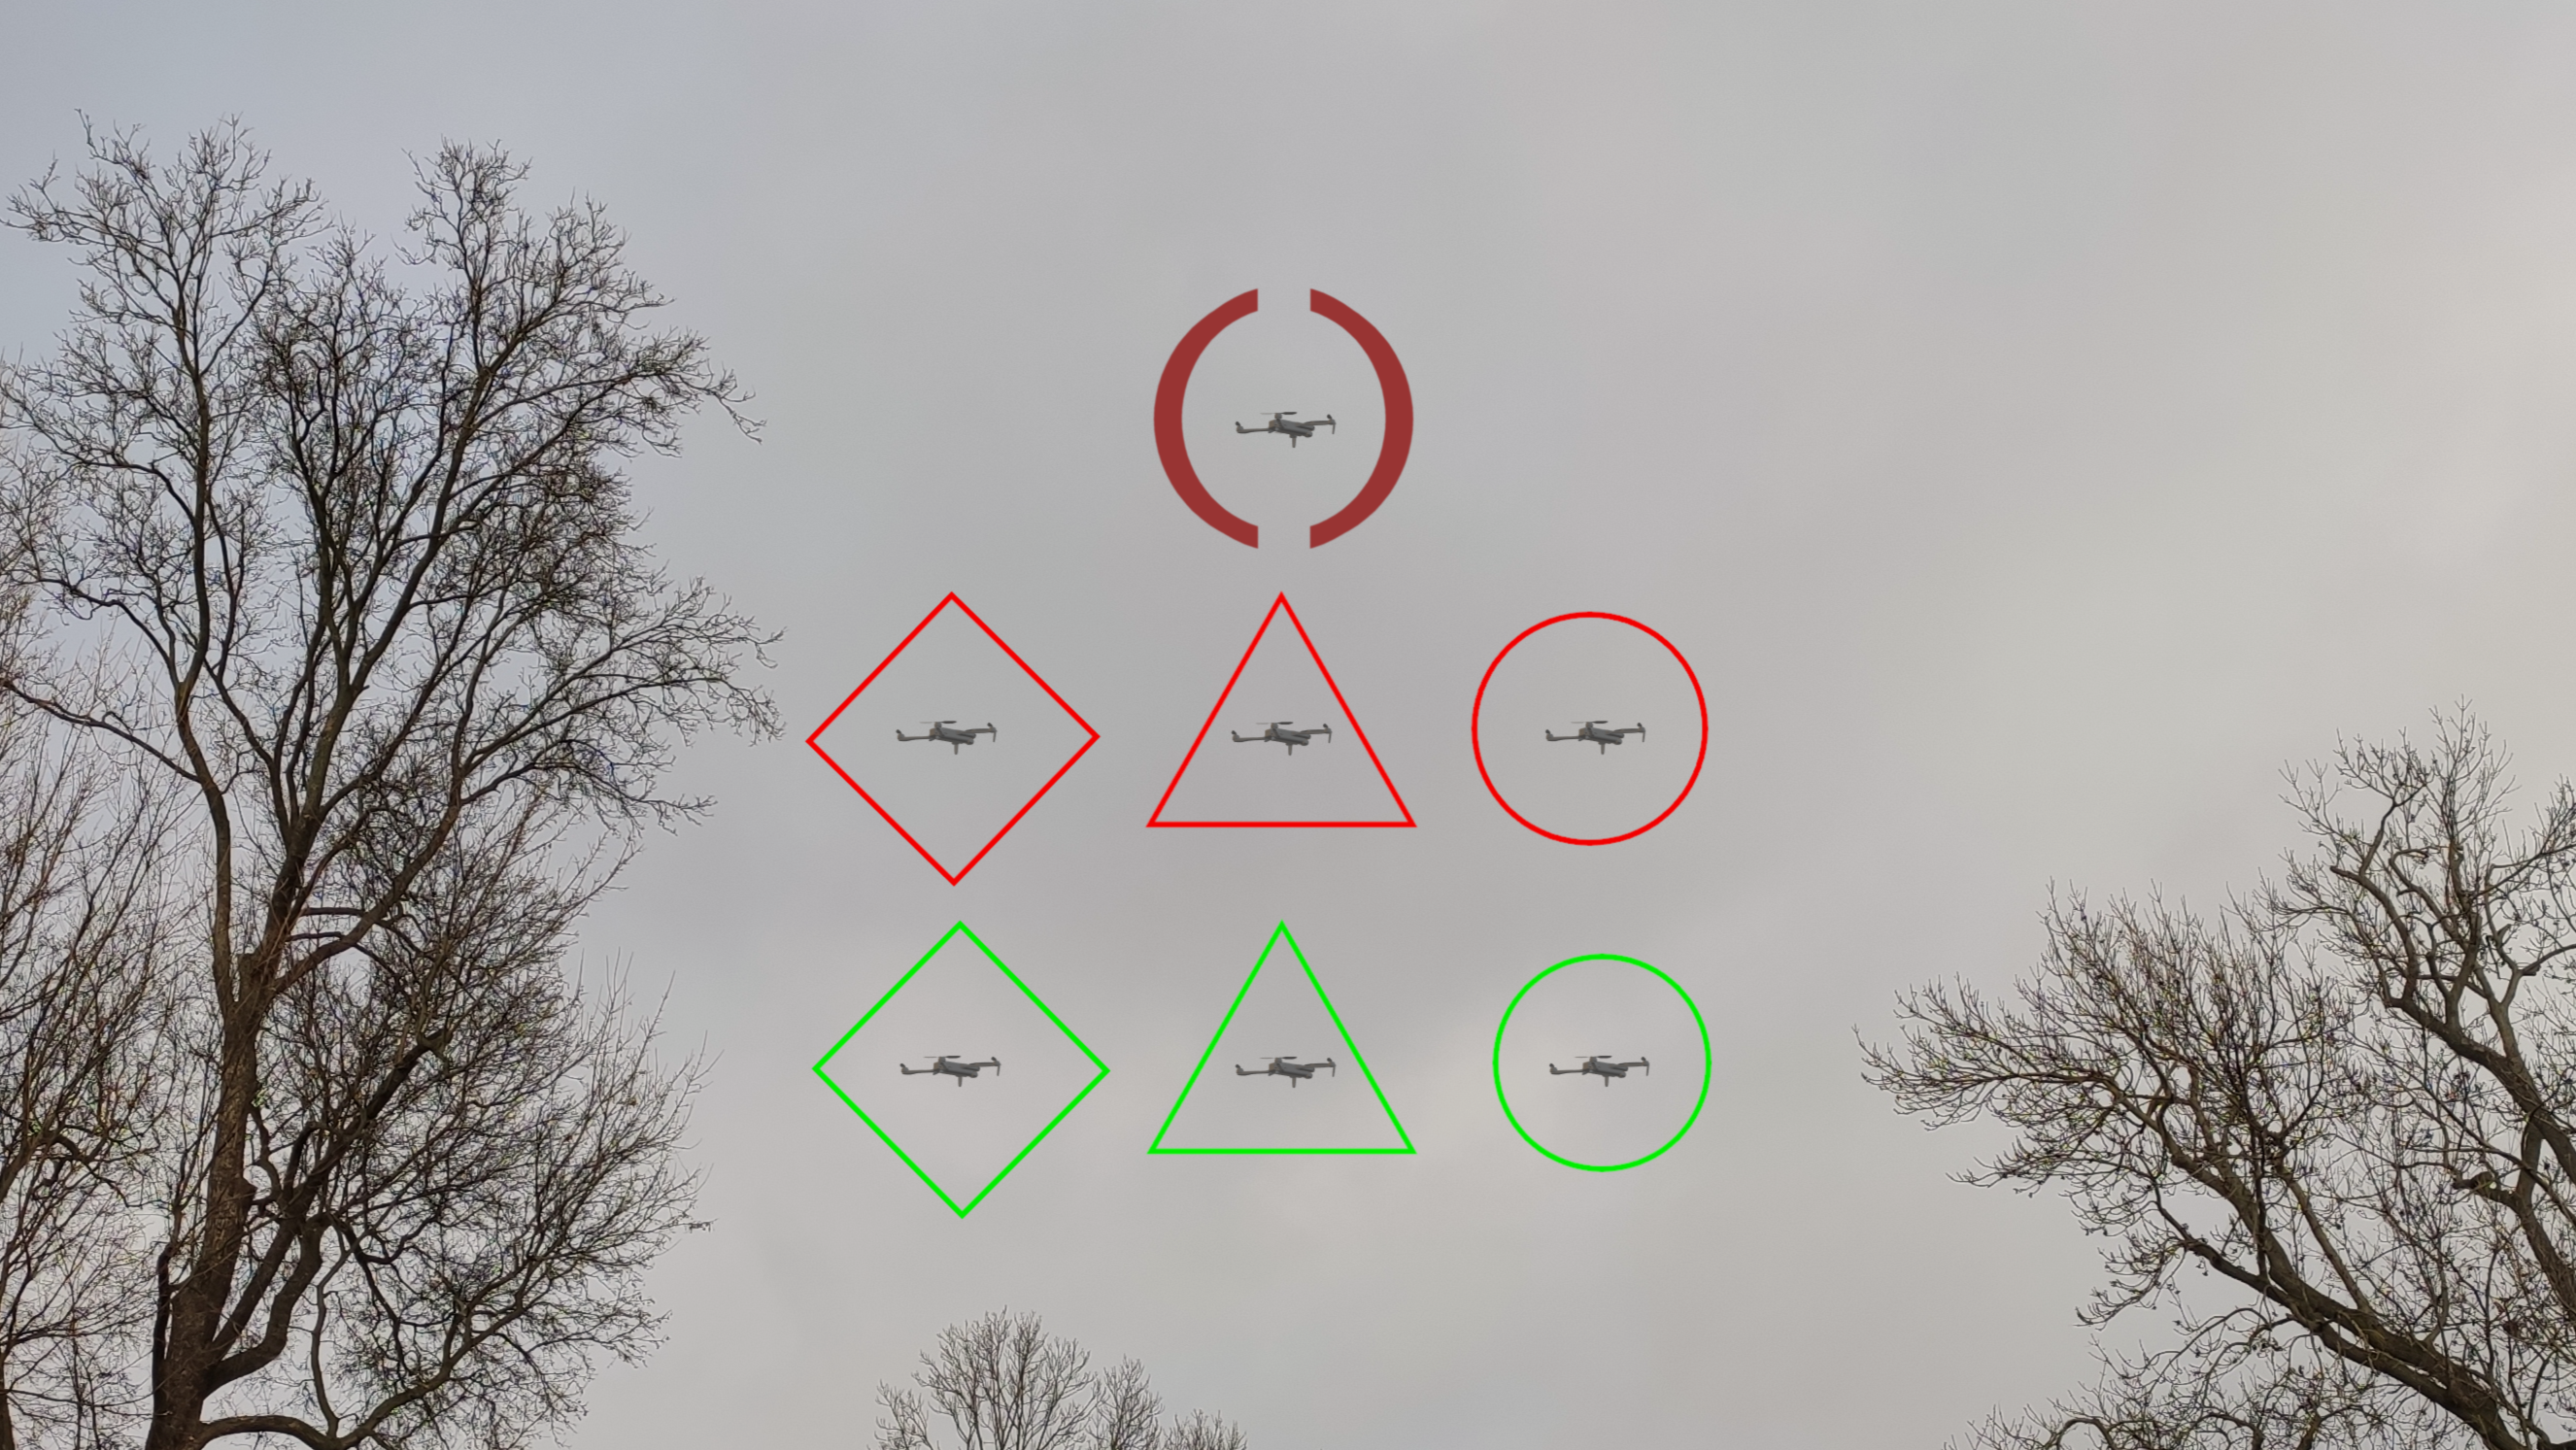
\includegraphics[width=\linewidth]{obrazky-figures/navrh/sledovaniDronaNavrhyCut.png}
    \caption{Provedený experiment s cílem najít nejlepší možné ohraničení dronu.}
    \label{pic:experimentOhraniceni}
\end{figure}
\subsubsection{Pohyblivá část rozhraní}
Pohyblivá část rozhraní z pohledu pilota sleduje dronu a ohraničuje ho. Tím má umožnit snadnější lokalizaci na obloze, pokud je dron v moc velké vzdálenosti od pilota. V rámci plenění cíle "minimalizace rozhraní" se autor rozhodl okolí dronu nechat prázdné a nechat zde pouze textový údaj vzdálenosti dronu od pilota.

Obrysový tvar byl vybrán díky experimentu, který je znázorněn na obrázku \ref{pic:experimentOhraniceni}. Jak je na obrázku znázorněno, v tomto experimentu figurovali různé obrazce, které autor opět vybral na základě předlohy HUD displejů.  Tentokrát se autor inspiroval u bojových letounů, které těmito obrazci indikují potencionální cíle v jejich zorném poli.  Nahoře tohoto obrázku se nacházel původní obrazec. 

Z důvodu, že zaměření dronu v původním řešení mělo potíže hlavně s vertikální složkou pohybu se autor rozhodl pro kosočtvercový tvar. Tento tvar přišel autorovy taky nejvíce esteticky líbivý. Zvolená barva byla již probrána ve statické části.  Integrace je vidět na kompozičním obrázku \ref{pic:ShowcaseNavrhBackView}.


\subsection{Návrh vizualizace navigačních údajů a prvků mise}
Tato část rozhraní má v první řadě za úkol lepší orientaci v prostoru. Autor se o proti původnímu řešení, které bylo určené pro let ve velmi blízkém okolí, rozhodl rozhraní uzpůsobit vzdálenějším letům. Obecným problémem u vzdálených objektů je rozpoznání vzdálenosti. Ilustrační příklad: ve vzdálenosti 40 metrů od pilota je strom a dronu máte poblíž, na první pohled nevíte jestli dron je před, za nebo vedle stromu. 

Z tohoto důvodu se autor rozhodl překážky a body mise nevkládat do prostoru na jejich fyzické místo. Místo toho se autor rozhodl vytvořit miniaturu okolí pomocí zmenšené 3D mapy, která bude přítomna před pilotem. Návrh je na obrázku  \ref{pic:MapaNavrh}. V základu by mapa měla podporovat vytyčení bez letové zóny, ta je v návrhu označena červeným polo transparentním kvádrem (v obrázku je umístěn na silnicí, nad kterou je dle legislativy zakázáno létat). Oranžová zóna značí zónu s omezením nebo varováním (na příkladu je takto vyznačen dvůr, kde by se mohli nacházet skupiny lidí, nad kterými se nesmí létat, zároveň by větší drony v této zóně měli létat v low-speed módu, aby jste nemusely létat ve vzdálenosti od lidí rovné letové výšce).

Dron je na obrázku vizualizován žlutě (pro odlišení od okolí žlutě). Nestandardním prvkem je přistávací zóna (modrá kulovitá plocha s nápisem "H"), která indikuje bod, na který se dron vrátí v případě výpadku signálu. Je zde i ilustrován uživatel.

Prvky mise jsou tvoří základní waypointy, kterými by se mělo prolétnout. Waypointy jsou propojené spojnicemi, takže lze plánovat celou kompletní trasu dronu. Díky 3D prostředí jsou na více viditelné zjevné kolize s budovami. Tuto vlastnost považuje autor za velmi přínosnou od konvenčních řešení v telefonech/tabletech. Plánovaná je i úprava prvků mise a to za pomocí fyzického přetahování a umisťování prvků do této minimapy. V návrhu bylo počítáno, že by jednotlivé typy objektů byly na kraji mapy, odkud by se zanášely do minimapy. V simulovaném scénáři by si mohl uživatel na základně naplánovat v prostředí brýlích celou misi, kterou by pak pouze v terénu pouze provedl.

Do prostoru je také umístěna obrazovka, která přehrává stream z kamery dronu. Původně se autor snažil tuto obrazovky umístit do statické části rozhraní, později i do dynamické, nicméně experimentálně bylo zjištěno, že tento způsob navozoval pocit nevolnosti při používání. Tato obrazovka je vidět na kompozičním fotu \ref{pic:ShowcaseNavrhBackView}.

\begin{figure}[!ht]
    \centering
    \includegraphics[width=\linewidth]{obrazky-figures/navrh/interaktiveMap.jpg}
    \caption{Ukázka návrhu interaktivní mapy prostředí.}
    \label{pic:MapaNavrh}
\end{figure}

\begin{figure}[!ht]
    \centering
    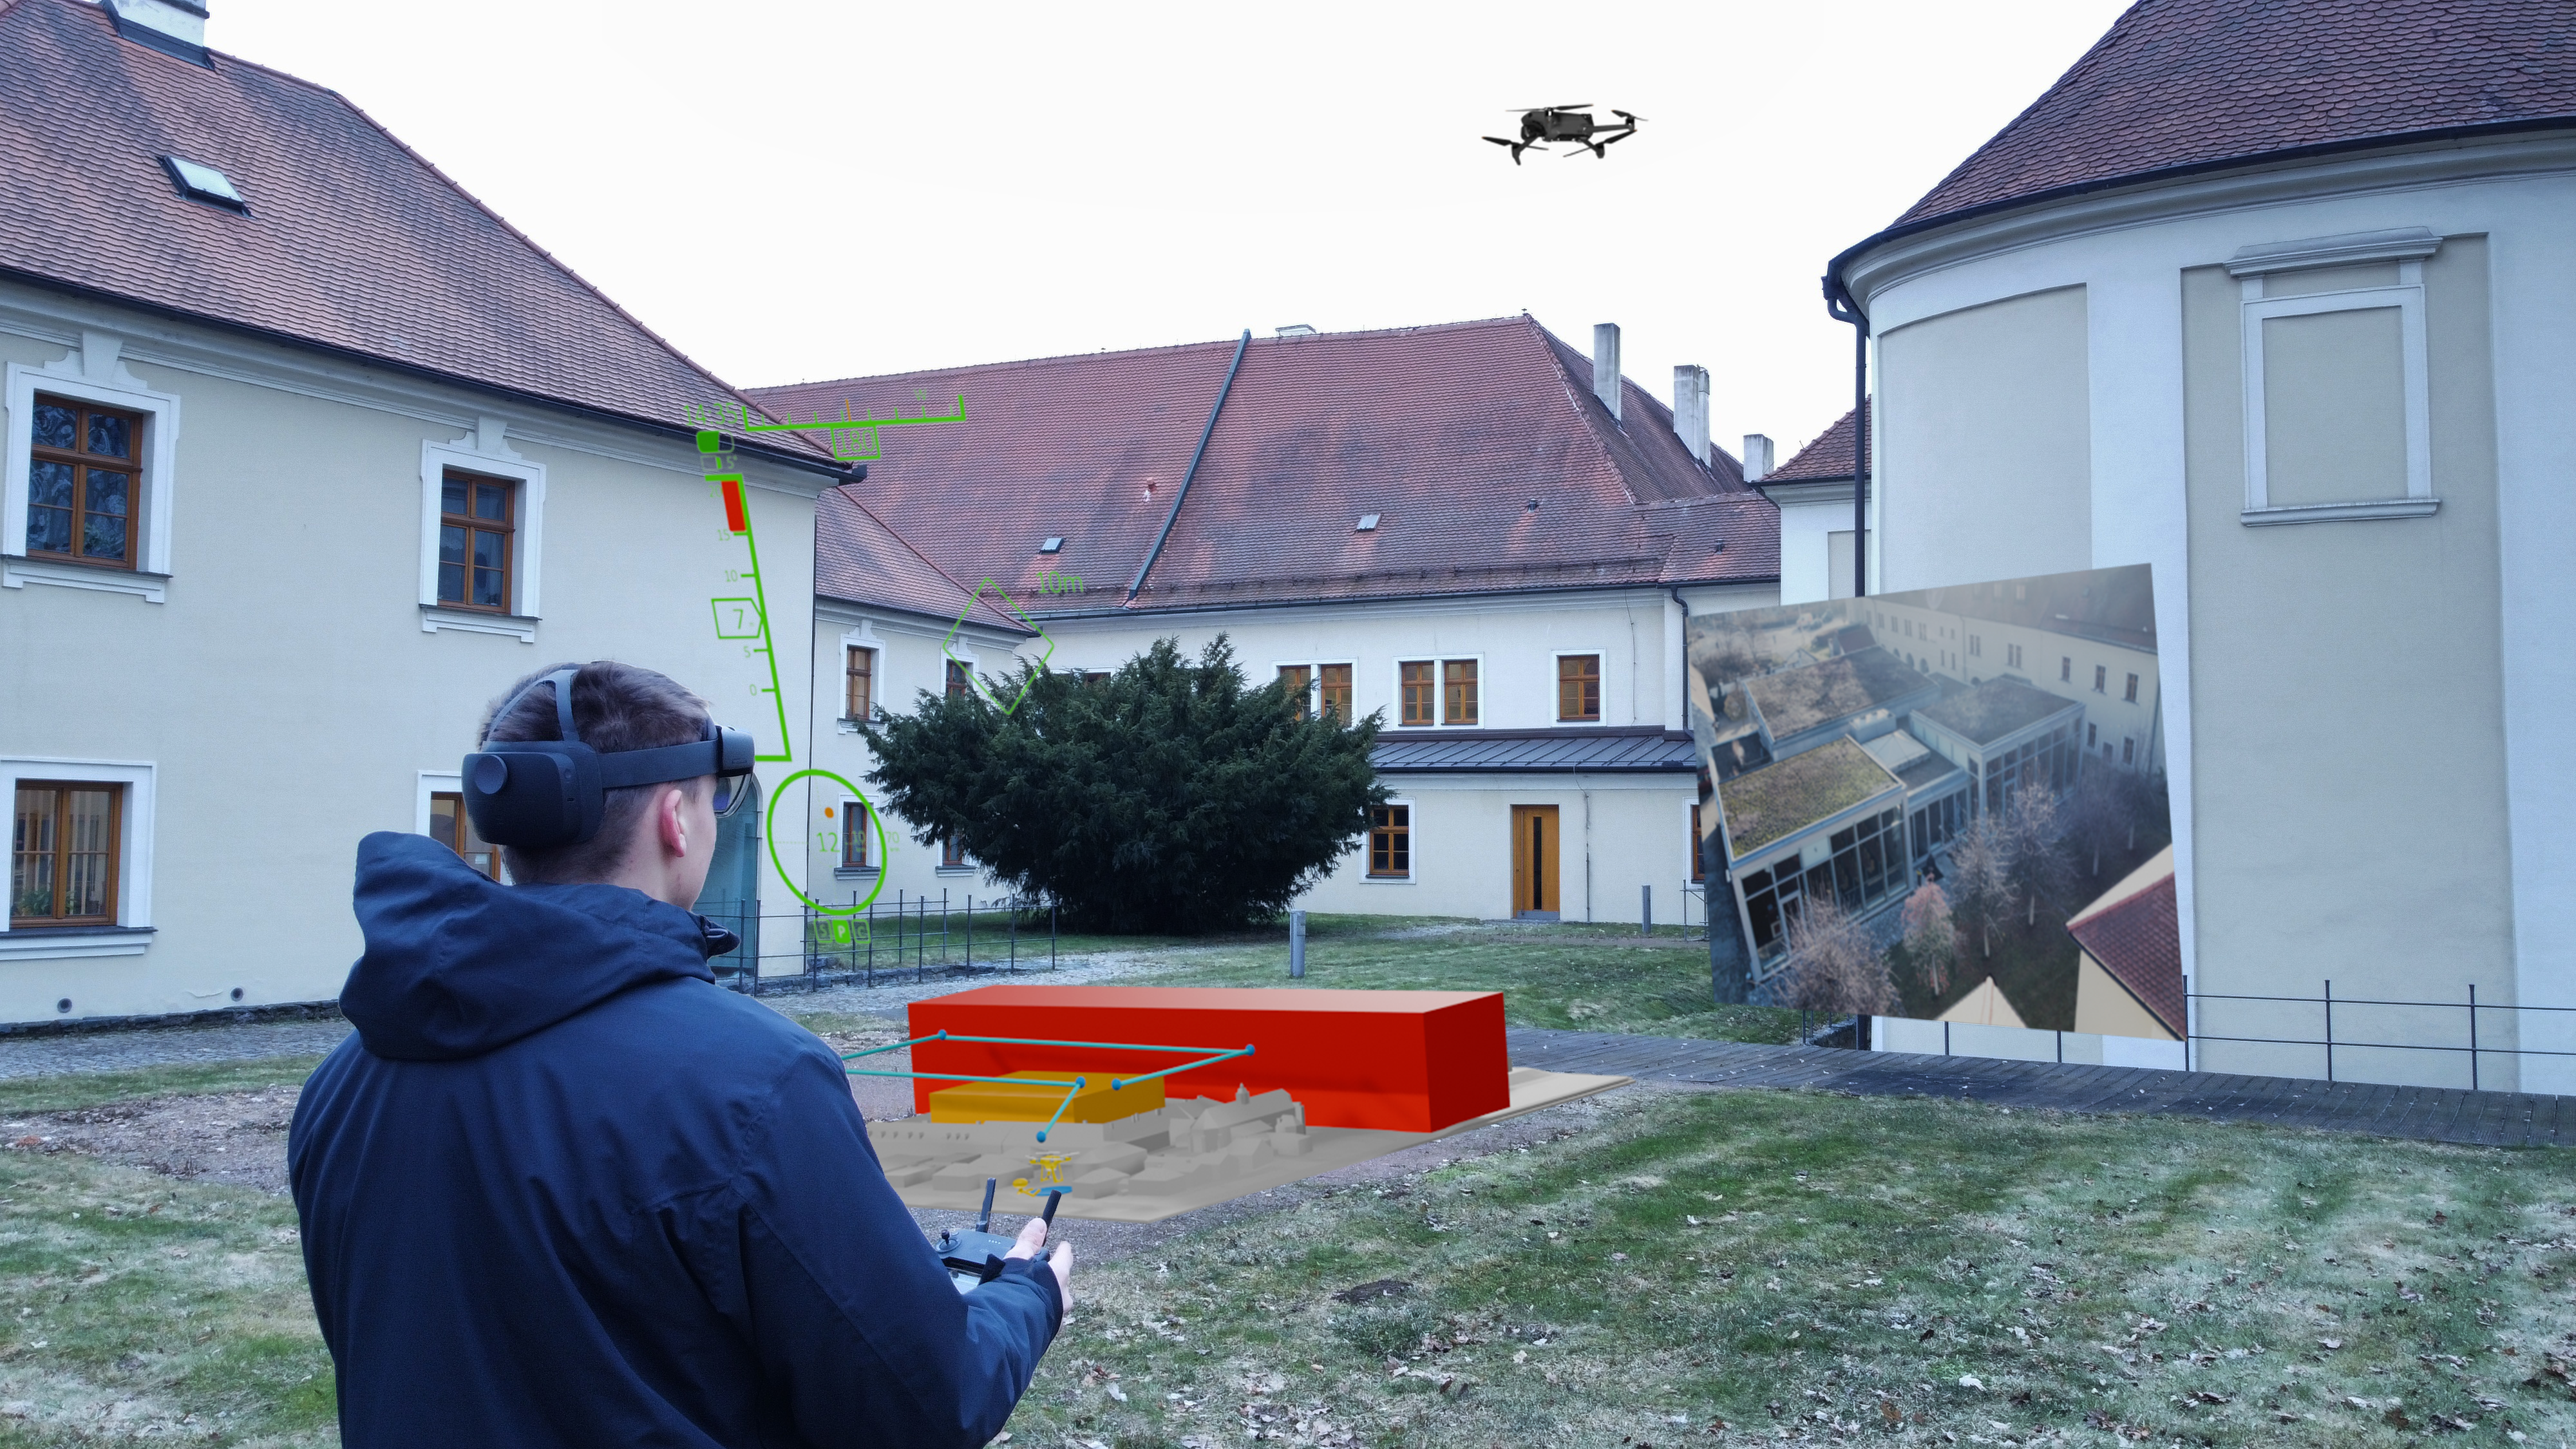
\includegraphics[width=\linewidth]{obrazky-figures/navrh/pohledZeZadu.png}
    \caption{Ilustrační foto, které ukazuje kompozici všech zmíněných částí rozhraní.}
    \label{pic:ShowcaseNavrhBackView}
\end{figure}


%\section{Zásady užité při návrhu}


\chapter{Implementace řešení}
Hlavní náplní kapitoly je realizace návrhu aplikace z předchozí kapitoly. Úvod kapitoly tvoří popis ekosystému v kterém má aplikace účinkovat. Součástí popisu je rozbor jednotlivých komponent, popis komunikace mezi nimi včetně popisu přenášených dat. Dále je navázáno představením technologií použitých při vývinu. Zbytek kapitoly je věnován detailnímu popisu implementačního procesu aplikace. Ten je rozdělen podle jednotlivých funkční modulů. Popis je doprovázen obrázkovou prezentací řešení.
\section{Architektura a komponenty systému } \label{sec:architektura}
Tato sekce se věnuje popisu celého ekosystému, který aplikace v brýlích potřebuje pro správné fungování. Systém bude nejdříve rozdělen a popsán podle jednotlivých komponentách. Na závěr bude nastíněna pravděpodobná hardwarová realizace v potencionální produkční verzi.

V systému účinkuje 7 komponent: Brýle, vysílač DJI\texttrademark, chytrý mobilní telefon, dron DJI\texttrademark, přístupový bod (dále již AP) a dvojice serverů (pro sběr a distribuci telemetrických dat a video streamů). Tyto komponenty jsou navzájem propojeny za pomocí různých přenosových technologií. Systém využívá serverového řešení z důvodu možnosti potencionálního budoucího rozšíření o integraci vizualizace více dronů či zapojení více operujících členů (například pozorovatelů).
Celý systém je vizualizován na obrázku \ref{pic:ekosystem}.
\paragraph{Popis jednotlivých komponent}
\begin{itemize}
    \item Brýle-- Již představené brýle Hololens 2 pro rozšířenou realitu (viz. \ref{sec:Hololens}), které bude mít pilot po celou dobu pilotáže pilot nasazené. Brýle potřebují ke své funkci spojení s dvojicí serverů, od kterých jsou distribuovaná telemetrická data a video přenos. Přenos do brýlí probíhá za pomocí WI-FI přenosu z přístupového bodu. Právě zde bude nasazeno vyvíjené rozhraní. 
   
    \item Vysílač  DJI\texttrademark-- Zajišťuje 3 hlavní funkce. První je bezdrátový přenos ovládacích instrukcí směrem k dronu a přenos telemetrických dat. K tomu využívá pásmo 2.4 GHz. Druhou funkcí je bezdrátový příjem video přenosu z kamery dronu. K tomu využívá pásmo 5 GHz. Oba zmíněné bezdrátové přenosy probíhají za pomocí proprietárních komunikačních technologií společnosti DJI\texttrademark. Třetí funkce ovladače je odesílání všech těchto dat do chytrého telefonu pomocí USB propoje. Více o vysílači viz. \ref{sec:ovladace}.
    
    \item Chytrý mobilní telefon -- Jedná se o libovolný mobilní telefon se systémem android kompatibilní s vysílačem, ke kterému je připojen pomocí USB. V tomto telefonu musí být nainstalována  aplikace Drone DJI Streamer\footnote{Odkaz na aplikaci Drone DJI Streamer: \href{https://github.com/robofit/drone\_dji\_streamer}{github.com/robofit/drone\_dji\_streamer}}. 

    
    Jedná se o upravenou verze aplikace DJI Fly\footnote{Aplikace DJI Fly je oficiální aplikace pro pilotáž dronu. Propojuje ovladač dronu s telefonem. Odkaz na aplikaci: \href{https://www.dji.com/cz/downloads/djiapp/dji-fly}{dji.com/cz/downloads/djiapp/dji-fly}  }, která je postavená na vydaném DJI SDK\footnote{SDK je soubor nástrojů, knihoven a dokumentace poskytovaných vývojářům pro snazší tvorbu aplikací. \\ Odkaz na DJI Android SDK: \href{https://developer.dji.com/mobile-sdk/downloads/}{developer.dji.com/mobile-sdk/downloads/}},  která zajistí distribuci telemetrických dat a video přenosu na patřičné servery. Uvažovaný způsob přenosu je pomocí technologie WI-FI přes přístupový bod. 
   
    \item Dron DJI\texttrademark \space -- Obyčejný, softwarově neupravený dron od firmy DJI\texttrademark, který komunikuje s vysílačem. V práci byl použit dron DJI Mavic 2 mini.
   
    \item Přístupový bod -- Zajišťuje propojení většiny koncových zařízení pomocí technologie WI-FI.
    
    \item Video server -- Zajišťuje příjem a distribuci RTMP streamů, které jsou vysílány z z aplikace mobilního telefonu. V práci je využita serverová aplikace MonaServer\footnote{Odkaz na open-source implementaci serverové aplikace pro streamování RTMP přenosů videa: \\ \href{https://github.com/MonaSolutions/MonaServer}{github.com/MonaSolutions/MonaServer}}, která podporuje řadu streamovacích protokolů, mezi kterými je i požadovaný RTMP protokol.
   
    \item Telemetrický server - Zajišťuje příjem a distribuci telemetrických dat. V práci je využit již implementovaný DroCo server\footnote{Odkaz na DroCo server, který zajičtůje přenos telemetrických dat: \href{https://github.com/robofit/drone_server}{github.com/robofit/drone\_server}}. Tento server je určen na provoz v kontejnerovém prostředí Docker\footnote{Docker je open-source platforma pro balení a  spouštění aplikací v izolovaném prostředí pro zajištění konzistentní funkčnosti nehledě na konkrétní platformu systému.}.
\end{itemize}

\begin{figure*}[ht]
    \centering
    \includesvg[width=\linewidth]{obrazky-figures/architektura.svg}
    \caption{Obrázek ukazuje jednotlivé komponenty architektury systému  a  jejich vzájemné propojení. K dispozici je i legenda ukazující technologii  propoje. }
    \label{pic:ekosystem}
\end{figure*}

\subsection{Přenášená data}

\paragraph{Telemetrická data} -- Přenášejí se mezi komponentami systému ve formátu JSON. Přenášejí se pouze nejnutnější data pro určení polohy, rychlosti pohybu a data pro režiji komunikace. Ukázka JSON dat viz. výpis \ref{drone-data-json}.
\paragraph{\textnormal{Popis jednotlivých údajů a veličin:}}
\begin{itemize}
    \item Client ID -- Jedná se o jedinečný identifikátor v rámci jedné sítě. Jeden dron má právě přiřazen jeden tento identifikátor. Aplikace v telefonu si při registraci na server tento identifikátor vygeneruje. Jedná se o 8 znakový hexadecimální řetězec.
    \item  Altitude -- Relativní výška dronu. Při startu dron předpokládá, že je ve výšce 0m. Potom pomocí akcelerometrů a optického senzoru odvozuje výšku, ve které se nachází. Znamená to, že pokud dron letí nad budovou, výška se nezmění.
    \item GPS souřadnice
    \begin{itemize}
        \item Latitude -- Zeměpisná šířka ve stupních.
        \item Longitude -- Zeměpisná délka ve stupních.
    \end{itemize}

    \item Údaje z gyroskopu -- Jsou posílány dvakrát. Ve formě dat z hlavního gyroskopu dronu a jednou z natočení gimbalu kamery. % to do ověřit fakty
    \begin{itemize}
        \item Pitch -- Náklon kolem osy  ve stupních, která prochází zleva doprava středem dronu. Indikuje náklon dopředu/dozadu.
        \item Roll --  Náklon kolem osy  ve stupních, která prochází zezadu do předu středem dronu. Indikuje náklon doleva/doprava.
        \item Yew -- Náklon kolem osy, která prochází z hora dolů  středem dronu. Indikuje otáčení dronu doleva/doprava.
    \end{itemize}
    \item Compass -- Udává kurz dronu ve stupních. Měl by se shodovat s údajem Yew.
    \item Údaje z akcelerometů -- Dron má v sobě implementovaný vlastní souřadnicový systém, jednotlivé rychlosti ukazují pohyb v tomto souřadnicovém systému nezávisle na otočení dronu. Popisované rychlosti platí pro rotaci (kompas) 0.
    \begin{itemize}
        \item Velocity X -- Rychlost v ose x (dopředná rychlost) m/s
        \item Velocity Y -- Rychlost v ose y (boční rychlost) v m/s
        \item Velocity Z -- Rychlost v ose z (vertikální rychlost) v m/s.
        %\item yaw_relative  - nevím co to je
     \end{itemize}
     \item Timestamp -- Časová značka pořízení dat.
\end{itemize}

\begin{figure}[ht]
  \begin{minipage}{0.5\textwidth}
    \begin{lstlisting}[ caption={Ukázka telemetrických dat ve formátu JSON.}, label={drone-data-json}]
{
  "client_id": "15357fc2",
  "altitude": 221.5,
  "gps": {
    "latitude": 49.227189718704956,
    "longitude": 16.59724337395506
  },
  "aircraft_orientation": {
    "pitch": 2.7,
    "roll": 0.7,
    "yaw": -113.8,
    "compass": -113.80000305175781
  },
  "aircraft_velocity": {
    "velocity_x": 0,
    "velocity_y": 0,
    "velocity_z": 0
  },
  "gimbal_orientation": {
    "pitch": 0,
    "roll": 0,
    "yaw": -122.5999984741211,
    "yaw_relative": 0
  },
  "timestamp": "2023-09-06 15:58:58.999"
}
\end{lstlisting}
  \end{minipage}%
  \hfill
  \begin{minipage}{0.45\textwidth}
    \centering
    \includegraphics[width=\textwidth]{obrazky-figures/gymbal.png}
    \caption{Vizualizace náklonů, které lze vyčíst z gyroskopu. Převzato z \cite{Flight-Control-dji}. }
    \label{pic:gymbal}
    \vspace{20pt}
    \includegraphics[width=\textwidth]{obrazky-figures/velocity.png}
    \caption{Vizualizace směrů rychlostí z akcelerometrů. Povšimněme si obrácené osy Z, která indikuje že rychlost při stoupání dronu je záporná. Převzato z \cite{Flight-Control-dji}.}
    \label{pic:velocity}
  \end{minipage}
\end{figure}
    
\paragraph{Video} - Video přenos z kamery dronu se přenáší za pomocí protokolu RTMP. Jedná se o protokol, který je používán pro přenos živého vysílání přes internet. Protokol rozděluje video stream do malých fragmentů, které následně posílá po síti. Protokol umí přenášet i audio stopu, pro tu však v práci není využití a proto je vypnuta. Tento protokol má přidělen TCP port 1935 a v čisté verzi není nijak zabezpečený\cite{RTMP}. 

Aplikace na telefonu dokáže zasílat živý přenos v HD rozlišení (1280x720 pixelů) při snímkovací frekvenci 30 snímků za sekundu. Užitý kodek je H264. Díky užití tohoto protokolu je zpoždění obrazu minimální.

\paragraph{Potencionální produkční implementace architektury}\mbox{} \\
Z předchozího popisu je patrné, že serverová část může být nasazena v internetu. Z praktického hlediska však tento přístup autor nedoporučuje kvůli velkým latencím při komunikaci a nepříliš velké variability v případě užití v terénu - řešení by bylo závislé na dosahu internetového spojení. 

Proto je uvažováno, že přístupový bod a obě serverové aplikace budou pravděpodobně integrovány v rámci jednoho systému a budou mít zajištěno externí napájení například z baterie. Celý tento systém by pak byl například umístěn do kufru pro přepravu dronu. 

\paragraph{Vývojové prostředí architektury}\label{par:vyvojProstredi}\mbox{} \\
V rámci vývoje byl  systém integrován na vývojovém notebooku, který zastal funkci jak serveru, tak přístupového bodu. K vývoji značně dopomáhal vizualizační nástroj  DroCo\footnote{Odkaz na aplikaci DroCo: \href{https://github.com/robofit/drone\_vstool}{github.com/robofit/drone\_vstool}}, který vizualizoval data z obou serverů.

\section{Užité softwarové prostředky a zdroje obsahu} 
Tato práce navazuje na předchozí práci \cite{KyjacMartin2022Vnpp} a proto se autor rozhodl pokračovat na již zavedených softwarových prostředích. Hlavním stavebním kamenem je engine/framework Unity. V tomto enginu je celý program vytvářen. Dále autor využil několika doplňků/knihoven do tohoto enginu. Struktura programu, hlavní doplňky a knihovny budou popsány dále v kapitole viz. \ref{SEC:StrukturaProgramu}. 
Na tvorbu 3D objektů byl využit modelovací nástroj Blender. Ke tvorbě statické vektorové grafiky posloužil nástroj InkScape viz. odstavec \ref{PAR:InkScape}.  
\subsubsection{Unity}
Unity je multiplatformní herní Engine, který byl představen roku 2005. Tento engine byl primárně vytvořen pro tvorbu 2D a 3D her. Postupným vylepšováním a rozšířením se z něho stal univerzální nástroj pro tvorbu programů využívajících funkcionalit jádra tohoto enginu . Integraci enginu tak můžete nalézt například v automotive průmyslu, architektuře a stavebnictví.  

Jeho veliká výhoda spočívá ve snadné integraci aplikací na různé typy platforem. Standardně tak lze unity použít pro vývoj aplikací pro desktopy, mobilní telefony (Android + IOS), herní konzole, brýle pro VR/AR a nově i pro aplikace na Webu. Engine tak musí podporovat řadu architektur výpočetních systémů, což je v případě brýlí Hololens 2 potřeba (platforma ARM)  \cite{unity1,unity2}. 
\paragraph{C\#}
Platforma Unity získala svou popularitu hlavně díky jednoduššímu a intuitivní stylu práce v tomto enginu. Jednoduché tvorbě dopomáhá jazyk C\#, který v enginu slouží pro psaní vnitřní logiky programu. Jedná se o vysokoúrovňový typovaný objektově orientovaný programovací jazyk. Tento jazyk lze mimo Unity nejčastěji nalézt v beckendové části Webových a formulářových aplikacích (.Net) \cite{cSharp}. 
\subsubsection{Blender}
Blender je open-source softwarový nástroj pro modelování 3D objektů, tvorbu animací a efektů. Kombinace Blenderu a Unity umožňuje bezproblémový přenos 3D objektů do herního prostředí s minimálním úsilím, což usnadňuje vývojový proces. V práci se využívá pro editaci a tvorbu 3D objektů, které následně jsou zaneseny do 3D scény v Unity \cite{blenderUnity,blender}. 

V Blendru se objekty nejčastěji modelují za pomocí mnoha propojených trojúhelníků v trojrozměrném prostoru. Trojúhelníky jsou základními stavebními bloky, které tvoří strukturu 3D modelů. Každý trojúhelník je definován třemi vrcholy, přičemž každý vrchol má své prostorové souřadnice. 

Při tvorbě se musí dát pozor na orientaci trojúhelníků, protože Unity kvůli optimalizaci nevykresluje trojúhelníky, které jsou orientované ke směru kamery \cite{blenderUnity}.
\subsubsection{Git a GitHub}
Pro udržení vývoje byla využit webová verzovací systém GitHub, který využívá systém zprávy verzí Git. GitHub poskytuje nástroje pro sledování změn v kódu, evidenci problémů, správu úkolů, diskusi a další. Ve spojení s Git umožňuje vývojářům snadno verzovat svůj kód, zaznamenávat změny a spolupracovat na projektech. V případě havárie lze změny zvrátit a navrátit se k předchozí funkční verzi kódu \cite{gitGithub}. 
\subsubsection{Chat GPT a Microsoft co-pilot}

\subsubsection{Github copilot}

\subsubsection{InkScape}

\subsubsection{Zdroje obsahu}
%
%
% https://sketchfab.com/3d-models/dji-mavic-3-c5a5abae1dea468ab73b1bdc7d616fa6#download
% https://www.svgrepo.com/vectors/dji/
\newpage
\section{Inicializační práce}
V této sekci budou stručně probrány úkony, které autor provedl v rámci inicializace projektového řešení. Jednalo se konkrétně o aktualizační proces, konfiguraci projektu a přechod na nový systém architektury.
\subsubsection{Migrace Unity a knihovny MRTK}
Původní projekt byl vytvořen ve starší verzi Unity 2019 a knihoven. Autor se z počátku pokusil v této verzi pokračovat a však různé chyby na předchozí platformě zamezovali další vývoj. Pro příklad integrace knihovny VLC nešla provést z důvodu kritických chybách v kolizi ve jmenném prostoru, tato a jiné chyby byly opravené v nové verzi Unity.  Proto se musela provést aktualizace. Po různých neúspěšných migračních pokusech celého projektu, se autor rozhodl pro čistou inicializaci projektu. 

Využita byla nejnovější stabilní verze Unity 2022. Na této nové verzi však nefungovala správně původní verze knihovny MRTK 2.4 (viz. sekce \ref{subsec:knihovny}), která je pro projekt esenciální. Autor se pokusil o aktualizaci na nový systém této knihovny, která je označena verzí 3.
Tato nová verze kompletně předělává systém integrace jednotlivých funkcionalit, protože jednotlivé funkce knihovny rozděluje do malých balíčkům čímž měla poskytnout lepší udržitelnost softwaru a snazší vývoj \cite{mrtk3}. Inicializace probíhala v této nové verzi bezproblémově. Bohužel je tato nová verze ve vývinu a některé funkcionality, které podporovala starší verze, nejsou ještě na integrovány. Konkrétně se jednalo o podporu vkládání objektů z Blendru, což byla hojně využívaná funkce v předešlé verzi. 

Tato a spousta dalších aspektů rozhodla, že nový systém knihovny ve verzi 3 nelze užít v aktuální projektu. Proto autor provedl inicializační proces znovu a to na poslední verzi starého sytému knihovny MRTK - 2.8.4. Tato verze se zdá být nejstabilnější (podle názoru autora). Vyřešila velké množství nekritických předchozích chyb v projektu, minimalizovala pády vývojového prostředí a pocitově vylepšila optimalizaci. 

\subsubsection{Konfigurace projektu}
Po předchozím procesu byl projekt inicializován dle následujícího návodu \cite{mrtk2TutorialInit}. Dodatečnými změnami byla úprava MRTK profilu pro vypnutí kolizí s okolním prostředím (aby byly hologramy vidět i když jsou "fyzicky" za stěnami či jinými překážkami). Toto nastavení usnadnilo vývoj. Dále bylo nutné MRTK profil přepnout do venkovního nastavení pro korektní fungování projektu.
\subsubsection{Přechod na nový ekosystém architektury}
Jak již bylo zmíněno, původní řešení komunikovalo s ovládacím chytrým telefonem na přímo proprietárním komunikačním protokolem. Tento protokol byl implementován ve skriptu "WebSocket Manager", vice viz. sekce \ref{SEC:StrukturaProgramu}.
Teto skript byl nahrazen novou implementací převzatou z programu, který vizualizoval stav telemetrického serveru (viz odstavec \ref{par:vyvojProstredi}). Tento skript byl modifikován autorem, aby přenášel do projektu data ve správném očekávaném formátu a byly zde přidány funkce odpovědné za korektní inicializaci při startu programu.
Mimo to bylo ještě nutné provést drobné úpravy spojené s vlastnostmi nové architektury. V první řadě se již nepřenáší typové označení dronu. Některé drony od DJI nepřenáší svoji relativní výšku, nýbrž odhadovanou nadmořskou výšku. To způsobovalo značné potíže v dynamické části rozhraní, která zaměřovala dronu. 

\section{Struktura implementovaného programu}\label{SEC:StrukturaProgramu}
Projekty v Unity se stávají z několika základních komponent. Tyto komponenty se poté umisťují do scény. Scéna je 3D prostor, kde se odehrává simulace. Jednotlivé komponenty  jsou standartě, v souborovém systému projektu, ve složce assets. Zde je několik základních typů souborů ve složce assets:

\begin{itemize}
    \item Scripts -- Obsahuje C\# skripty, které obsahují vnitřní logiku programu.
    \item Prefabs -- Jedná se o zapouzdřené celky objektů, které jsou vytvářeny pro co největší znovupoužitelnost.
    \item Materials -- Obsahuje materiály objektů, které ovlivňovat vzhled a textury objektů.
    \item Textures -- Tento adresář může obsahovat textury pro objekty ve hře.
    \item Models -- Obsahuje 3D modely pro objekty ve vaší hře. Zde jsou umisťovány modely z programu Blender.
\end{itemize}

\subsubsection{Struktura implementovanému Unity projektu}
Nyní bude probrána konkrétní struktura implementovaného projektu. Celé rozhraní je umístěno v jedné hlavní scéně označené názvem "Main". Obrázek \ref{pic:unity} obsahuje otevřenou scénu, ke které se vztahuje popis. V této scéně je umístěno následující:
\begin{itemize}
    \item Diractional Light -- Zavádí všesměrové osvícení scény. 
    \item MixedReality Toolikt -- Obsahuje konfigurační skripty pro integraci na HoloLens 2.
    \item MixedRealityPlayspace -- Obsahuje speciální MRTK kameru. Tato kamera představuje hráče. V projektu jsou zduplikovány a rozděleny pro pravé a levé oko z implementačních důvodů.
    \item Settings -- Obsahuje konfigurační menu umístěné do prostoru, pro nastavení parametrů interní logiky programu.
    \item StaticHud --  Obsahje statický HUD.
    \item Managers -- Zde jsou jednotlivé skripty odpovědné za připojení k serverům, evidence připojených dronů a jejich následné umístění do scény.
    \item Scene Manager -- Obsahuje dynamickou část rozhraní, které zaměřuje dronu.
    \item Controlled Drone --  Virtuální reprezentace ovládaného dronu.
    \item Map -- Mapbox mapa pro evidenci GPS údajů z dronu.
    \item Hand Menu -- Malé ovládací menu, které slouží pro umístění hlavních ovládacích tlačítk, včetně tlačítka pro vyvolání velkého meny v "Settings".
    \item Debug Console -- Výpisy ladící konzole pro účely ladění přímo v Hololens brýlích.
    \item VLC -- Obsahuje displej s integrací VLC přehrávače, který zobrazike  RTMP stream z dronu. Obsahuje  
\end{itemize}

\subsubsection{Užité knihovny}\label{subsec:knihovny}
Projekt využívá několik přídavných Unity balíků. Tyto balíky lze nainstalovat automaticky do projektu díky Unity Paket manageru. Balíky lze instalovat z oficiálního zdroje, ty jsou v Unity registru nebo lze užít možnost instalace skrze adresu GitHub repositáře. Balíky neumožnující tuto možnost se musejí instalovat manuálně pomocí import nástroje a jejich aktualizace se musejí provádět taktéž manuálně.

\begin{itemize}
    \item \textbf{Abstract websocket} -- Tato knihovna byla v projektu užita pro otevření síťového soketu, kterým se komunikuje se serverem distribuující letová data.
    \item \textbf{VLC for Unity} -- Poskytuje rozhraní pro přehrávání mediálních souborů, včetně RTMP realtime streamů. Jedná se o placenou knihovnu, která má zkušební verzi s plnou funkcionalitou knihovny, ale s vodoznakem. Proto je na implementačních obrázcích v dolním rohu nápis.\todo{Zmínit nákup licence :D}
    \item \textbf{MRTK} -- Jedná se o oficiální knihovnu od Microsoftu, které velice usnadňuje vývoj pro brýle Hololens. Poskytuje asistenci při konfiguraci projektu a celé Unity scény. Spolu s knihovnou jsou dodány pomocnými prefabrikáty, jako jsou například UI elementy. Další funkcionalitou podporující vývojový cyklus je remote play, díky které je možné streamovat obraz do brýlí z vývojového PC.
    \item \textbf{Balík SVG} -- Přidává experimentální podporu pro vektorovou 2D  grafiku.
    \item \textbf{Mapbox} -- Umožňuje práci s mapou. Tuto mapu lze vnést do scény v různé podobě. Podporuje i vizualizaci 3D terénu.
    \todo{Zmínit upravená dll}% https://github.com/mertusta1996/Mapbox-Hololens-2-Unity-UWP-
    \item \textbf{ProBuilder} -- 
\end{itemize}
\begin{figure}[H]
    \centering
    \includegraphics[width=1\linewidth]{obrazky-figures//implemetace/unity.png}
    \caption{Ukázka projektu v Unity. Na pravé straně jsou vidět veškeré hlavní komponenty řešení.}
    \label{pic:unity}
\end{figure}
\newpage
\section{Ladící a optimalizační nástroje}
\subsubsection{MRTK profiler}
\subsubsection{Unity profiler}
\subsubsection{Vlastní ladící nástroje}
Brýle Hololens neobsahují žádné ladící výstupy a vstupy, proto si autor některé vlastnoručně vytvořil. Jedním z hlavních byla ladící konzole, která ke vyobrazena na obrázku \ref{pic:debugConsole}. Tato konzole byla vytvořena z důvodu ladění implementace na cílové platformě. Ve vývoji bylo kvůli větší pohodlnosti použit přístup streamování obrazu přímo do brýlí, který však neodpovídal plně reálnému stavu po nasazení do brýlí. Konzole obsahuje jednoduchý canvas, na kterém je textové pole TextMash Pro. Komponenta obsahuje skript, který přesměrovává vybrané typy logů v konzoly do tohoto textového pole.
\begin{figure}[H]
    \centering
    \includegraphics[width=1\linewidth]{obrazky-figures//implemetace/debugConsole.jpg}
    \caption{Vytvořený ladící nástroj -- vývojová konzole, která lze přesouvat a zvětšovat gesty.}
    \label{pic:debugConsole}
\end{figure}

\section{Implementace jednotlivých modulů}
V této kapitole budou obsaženy informace ohledně implementace jednotlivých komponent.


\begin{figure}[ht]
    \centering
    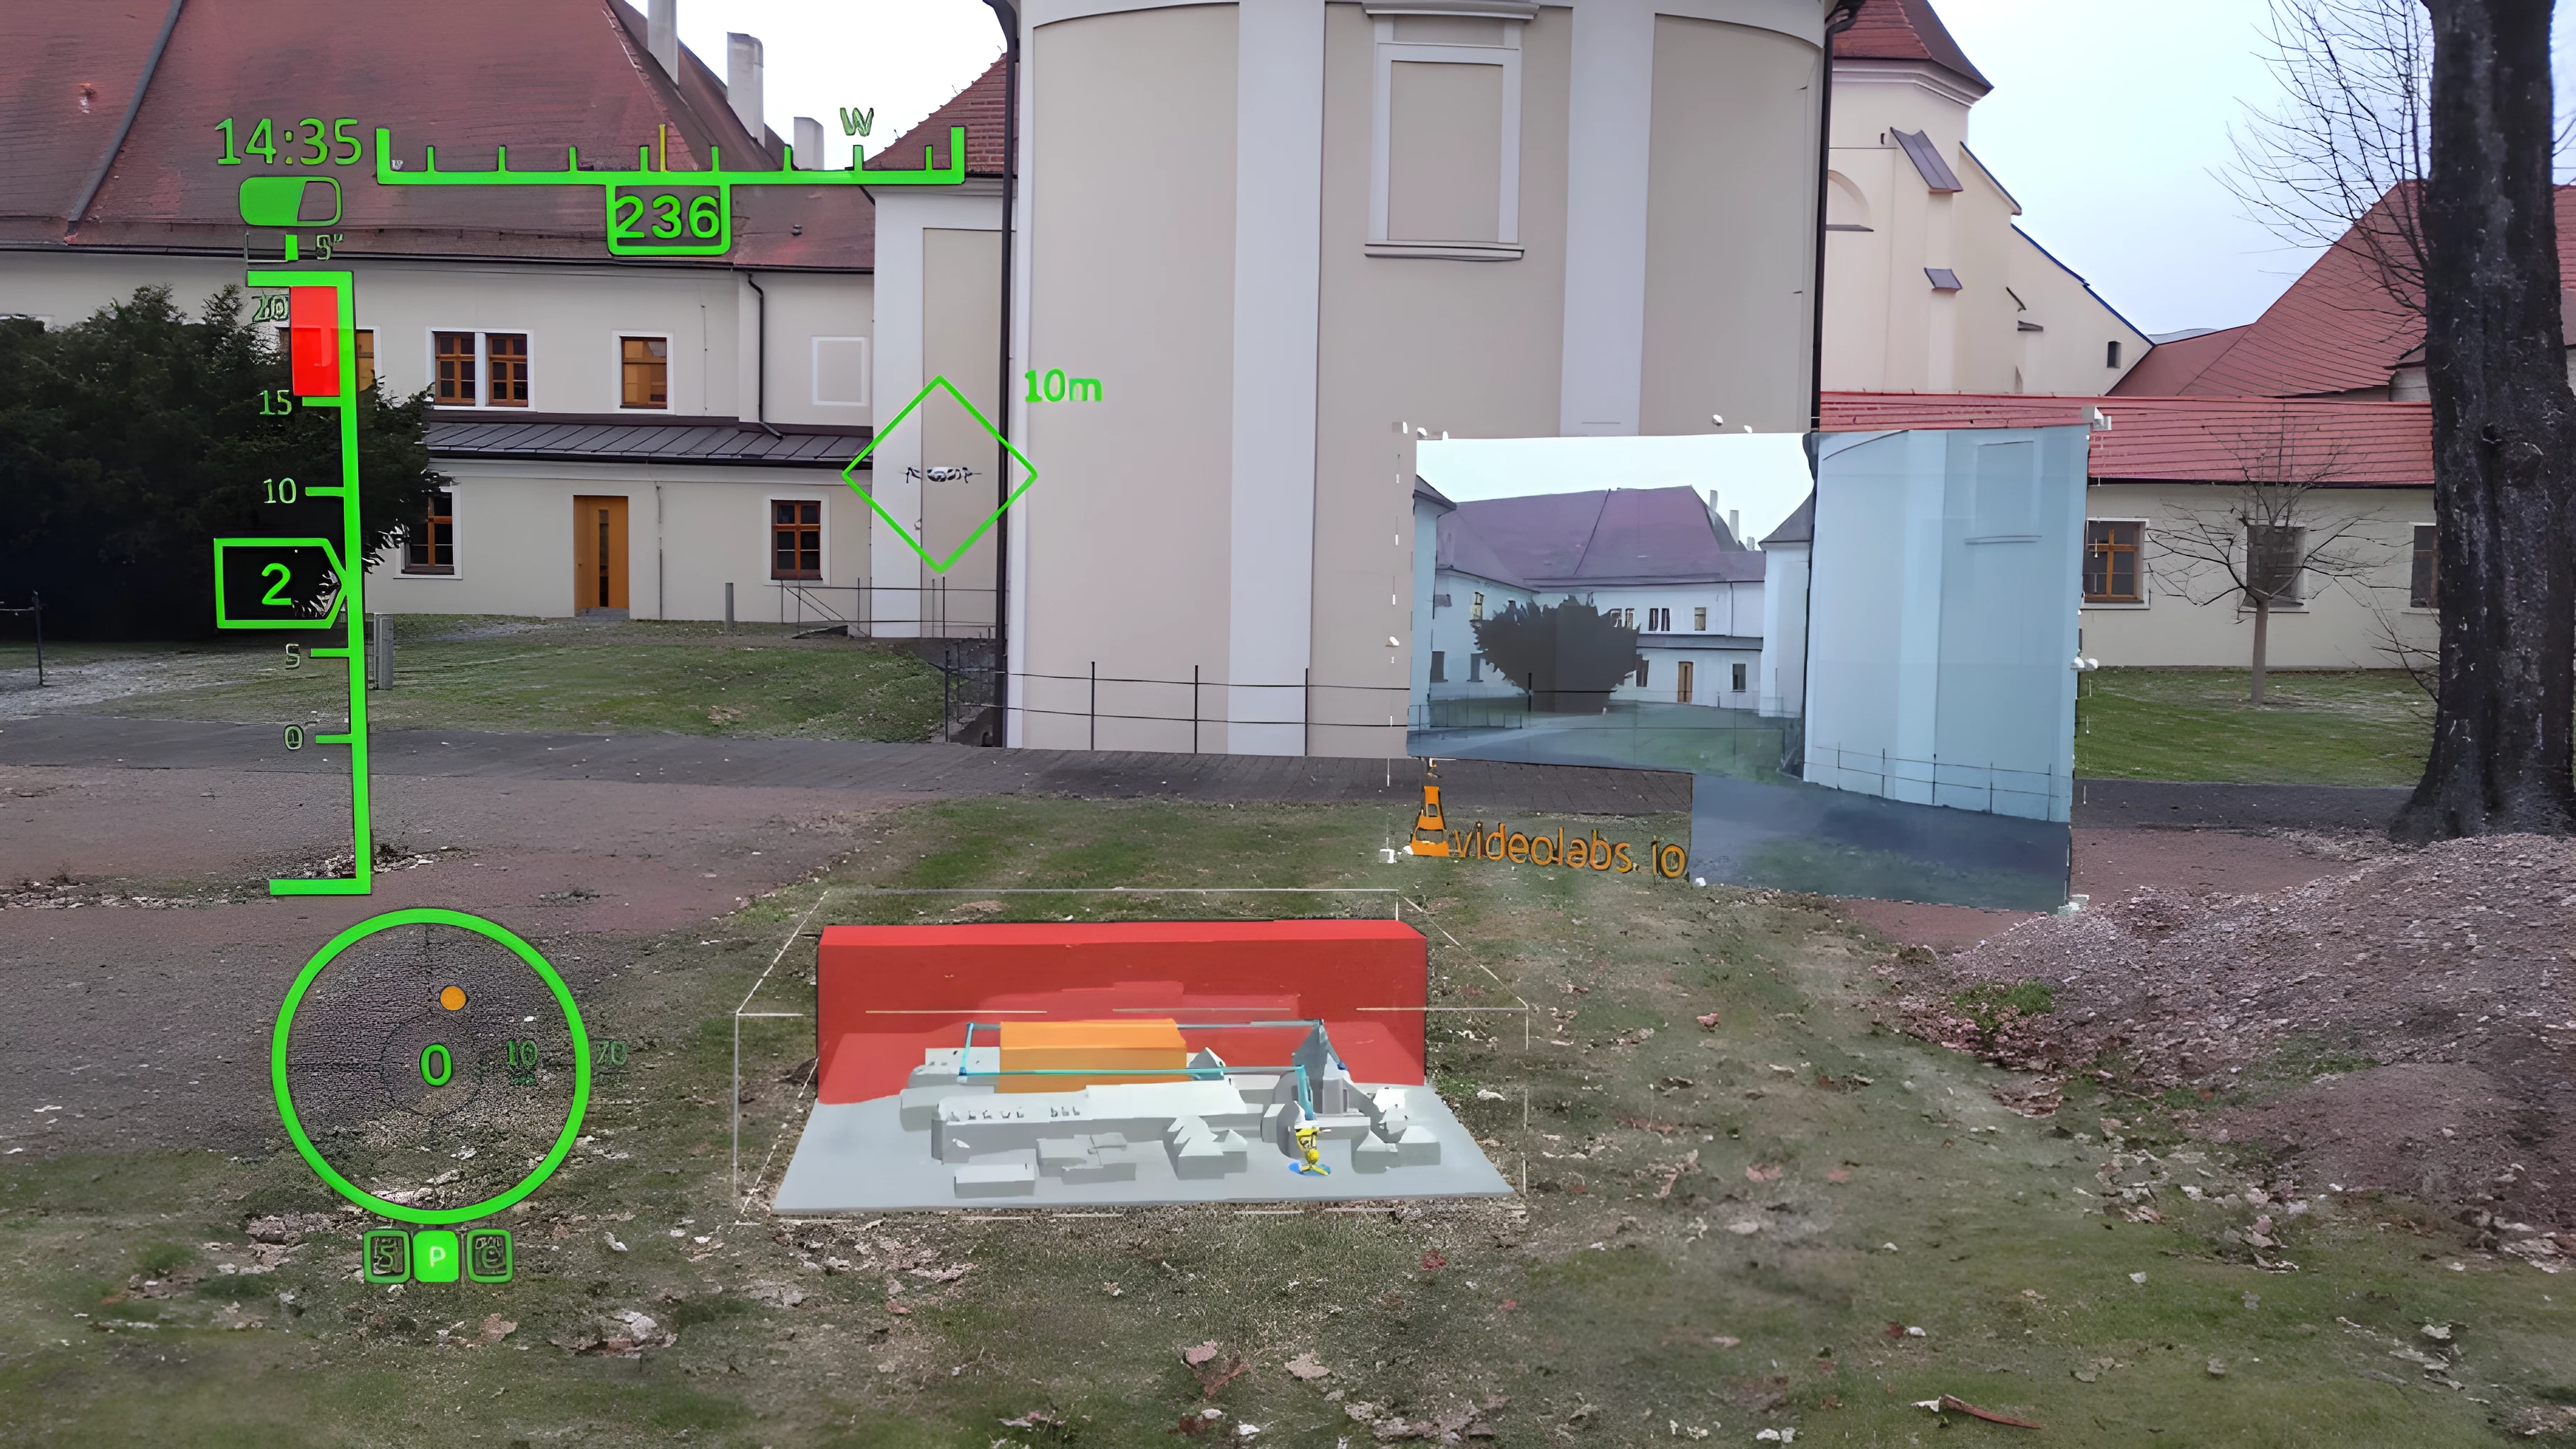
\includegraphics[width=1\linewidth]{obrazky-figures/implemetace/pohledZHololensAiAugmented.png}
    \caption{Ukázka demonstrační implemetace v Unity pro experimentální účely vyfocenou skrze brýle Hololens 2. (obrázek byl post-produkčně vylepšen). }
    \label{fig:progress}
\end{figure}

\subsection{Implementace HUD a sledování pozice dronu}
% ukázat, že jsem udělal rozhraní z návrhu, vysvětlit proč stálo za prd

\subsubsection{Statická část - vizualizace hlavních letových veličin}
\subsubsection{Dynamická část - sledování pozice dronu}



\subsection{Implementace vizualizace prvků mise}

\subsubsection{Minimapa}

\subsubsection{Wordscale mapa}



\subsection{Zajištění persistence dat \& mission manager}
\section{Optimalizace}
% mapbox  - snížení dosahu wordscalu a vypnutí mlhy, užití korutin, snížení kvality map
% vlastní kód - implementace korutiny na pozici spawnu, redukce update funkcí - otimalizace detekce kolizí přes eventy
% vlc - displeje vypnuty, zapínajíse pouze pokud jsou potřeba - šetření datového toku
% redukce objektů ve scéně
% grafické nastaveí - vypnutí antialiazingu, optimalizace textur
%

\chapter{Experimenty a uživatelské testování prototypu}

\section{Testovací scénáře}

\subsubsection{Filmaři}
\subsubsection{Inspekce fasády budovy}
\subsubsection{Inspekce solárních panelů}

\section{Měřené veličiny}
\subsubsection{Čas}
\subsubsection{NASA-TLX}
\subsubsection{Vyhodnocení splnění úkolu}
\subsubsection{Formulář použitelnosti}
\subsubsection{Doplňkové otázky}

\paragraph{Hud}
\paragraph{Minimapa}
\paragraph{Objekty ve scéně}
\section{Zhodnocení výsledků}
\section{Rozprava o možných budoucích směrech v daném odvětví}
\chapter{Závěr}
Začátek práce je tvořen obeznámením s rozšířenou realitou. Dále jsou představeny brýle Hololens 2. Popsány jsou zejména modality vstupu brýlí a technické limitace brýlí. Téma další kapitoly byl drony a jejich bezpečný provoz dle legislativy. Navázalo se návrhem rozhraní v rámci kterého byla provedena analýza původního řešení. Poté následoval soupis požadavků nového rozhraní a stanovení cílů rozhraní. Dále bylo rozhraní navrhnuto pomocí drátových modelů a detaily doladěny v grafickém modelu. 

Závěr semestrálního projektu tvoří začátek implementační fáze projektu, kde byla prezentována architektura celého systému v rámci které byly popsány data, která se mezi jednotlivými systémy přenáší. V další sekci se již probíraly prostředky použité k vývoji. Poté byla od prezentována struktura programu, za kterou následoval popis implementace jednotlivých částí programu. 

V rámci pokračování práce chce autor dodělat všechny moduly popsané v návrhové části. Celý program chce autor uživatelsky otestovat, aby se ověřilo splnění cílů rozhraní udaných v návrhové části. Pro toto testování autor plánuje vytvořit testovací scénář v rámci kterého bude testovaný provádět řadu letových úkonů. Na konci testu bude testovaný vyplňovat řadu formulářů, mezi kterými bude NASA-TLX. Autor v rámci testování také chce měřit metriky jako je čas provádění úkonů a přesnost. Závěr diplomové práce má tvořit reprezentace výsledků testů a zodpovězení otázky, zadali technologie rozšířené reality má potenciál v tomto technologickém odvětví.
